% ============================================================================
% Paper 1 -- converted to LaTeX from the published article (J. Biomed. Inform. 178 (2026) 105022, PDF supplied in
% papers/1-s2.0-S1532046426000468-main.pdf). No Word version of the paper was supplied. Generated by a conversion
% script from the PDF text layer; see the integration report for the conversion procedure and known issues.
% ============================================================================
\section{Challenges of health data standard adoption and usage: a systematic review}
\label{sec:paper1}

\noindent This section contains the article~\cite{marfoglia2026challenges}.

\paragraph{Authors.}
Alberto Marfoglia\textsuperscript{a}, Valerio Antonio Arcobelli\textsuperscript{b,*}, Serena Moscato\textsuperscript{b}, Antonino Amedeo La Mattina\textsuperscript{c}, Sabato Mellone\textsuperscript{b}, Antonella Carbonaro\textsuperscript{a}

{\raggedright % layout: ragged-right metadata block
\noindent\textsuperscript{a}Department of Computer Science and Engineering - DISI, University of Bologna, Via dell'Universit\`a 50, 47521 Cesena, Italy\\
\textsuperscript{b}Department of Electrical, Electronic and Information Engineering ``Guglielmo Marconi'' -- DEI, University of Bologna, Viale del Risorgimento 2, 40136 Bologna, Italy\\
\textsuperscript{c}Medical Technology Lab, IRCCS Istituto Ortopedico Rizzoli, Bologna, Italy\\
\textsuperscript{*}Corresponding author. E-mail address: valerio.arcobelli2@unibo.it (V.A. Arcobelli).\\
Journal of Biomedical Informatics 178 (2026) 105022. \url{https://doi.org/10.1016/j.jbi.2026.105022}. Received 28 August 2025; Received in revised form 29 January 2026; Accepted 17 March 2026; Available online 21 March 2026. 1532-0464/\textcopyright{} 2026 The Author(s). Published by Elsevier Inc. This is an open access article under the CC BY license (\url{http://creativecommons.org/licenses/by/4.0/}).
\par}

\subsection*{Abstract}

Objective: To explore the adoption and practical implementation of the three major health data standards (i.e., FHIR, OMOP-CDM, and openEHR), to evaluate their maturity level in terms of how extensively they have been applied and integrated into everyday clinical and research practice.\\
Methods: We conducted a systematic review registered in PROSPERO (CRD42024623398) following PRISMA guidelines. Literature searches were performed through PubMed, Cochrane, Scopus, Web of Science, and IEEE Xplore from 2021 to 2024. After de-duplication and screening, 99 studies were included. Data was extracted and classified according to five health application domains and five use cases based on the intended purpose of the standard in the work. Studies were assessed for implementation scale, ETL tools, coverage of the standard (i.e., the number of mapped source variables), and whether standards were adapted or used as-is.\\
Results: Of the 99 included studies, 57\% used OMOP-CDM, 39\% FHIR, and 8\% openEHR. Most applications occurred in research settings (87\%) and focused on data reuse (47\%) or clinical decision support (23\%). OMOP-CDM was preferred for large-scale, longitudinal research, while FHIR was dominant in the public health domain and for real-time data exchange. Only 27\% of studies reported the coverage of the standard. FHIR implementations often require customization, complicating interoperability. OMOP-CDM offered strong analytical tooling but posed challenges for mapping and data loss. Few studies using openEHR reported limitations, with its uptake remaining limited.\\
Conclusion: Although FHIR, OMOP-CDM, and openEHR hold significant potential to enhance interoperability, their adoption remains fragmented. Each standard shows specific strengths: FHIR for exchange, OMOP-CDM for analytics, and openEHR for data persistence. A hybrid approach and clearer implementation practices are essential to support scalable, interoperable health data ecosystems.

\paragraph{Keywords:} Health data standard; Interoperability; Health informatics

\begin{table}[htbp]
\centering
\begin{tabular}{p{0.28\textwidth} p{0.62\textwidth}}
\hline
\textbf{Problem or Issue} &
Despite growing availability of health data standards, their real-world adoption remains fragmented, and the maturity and integration of the major health data standards (i.e., FHIR, OMOP-CDM, and openEHR) are not well characterized.
\\[0.5em]
\textbf{What is Already Known} &
FHIR, OMOP-CDM, and openEHR each support specific aspects of health data interoperability. Existing literature focuses mostly on isolated implementations or theoretical comparisons, without mapping actual usage.
\\[0.5em]
\textbf{What this Paper Adds} &
This paper systematically reviews 99 studies to assess how, where, and why these standards are used in real-world settings. It identifies gaps in ETL reporting, extension practices, and proposes a hybrid ecosystem model.
\\[0.5em]
\textbf{Who would benefit from the new knowledge in this paper} &
Health informatics researchers, standard developers, policymakers, and system integrators seeking to improve interoperability and guide informed standard adoption across healthcare and research domains.
\\
\hline
\end{tabular}
\end{table}

\subsection{Introduction}
\label{sec:paper1_introduction}

The healthcare industry generates about 30\% of the world's data volume \cite{thomason_data_2024} from various sources \cite{leavy_data_2019}, including electronic health records (EHRs) \cite{wang_electronic_2023}, administrative information \cite{cadarette_introduction_2015}, laboratory systems \cite{harrison_role_2008}, imaging systems \cite{noauthor_medical_2018}, medical devices \cite{moscato_wrist_2022,arcobelli_enhancing_2024,arcobelli_mcrutch_2023}, and consumer devices \cite{piwek_rise_2016}. In this scenario, data standardization has garnered significant attention in recent years as a pivotal step to efficiently exploit this precious source of information. The widespread adoption of standards in various applications, such as clinical trials, hospital information systems, and public health data streams, provides significant enhancements in communication and optimization of patient care workflows \cite{pimenta_interoperability_2023}. By leveraging seamless exchange and sharing of data, standardization enables continuity of care across all levels of the health system, independently of the specific software in use \cite{torab-miandoab_interoperability_2023}. Moreover, the adoption of a standardized framework for healthcare data interoperability offers significant benefits for the secondary use of real-world data in medical data science, including cost efficiency, improved data quality, and exceptional analytical flexibility \cite{gehrmann_what_2023}.

Despite the promising aspects of the health data standard adoption in clinical settings, there are still some concerns about its widespread use. The main challenges are political and technical. The former category, being among the most difficult obstacles to overcome \cite{shankardass_implementation_2018}), primarily arises due to an extreme heterogeneity in local policy adoption, often lacking a ``Health in All Policies'' approach \cite{noauthor_health_2006} fostering cross-sector collaboration to achieve common goals in the health domain; policy fragmentation is exacerbated by the frequent policy changes implemented to address public health issues. On the other hand, technical challenges result from the heterogeneous landscape of architectures, formats, applications, tools, and vendors that have independently contributed to the development of information systems across hospitals, healthcare organizations, and research institutions. In this context, concerns persist regarding the large-scale adoption of Extract, Transform, Load (ETL) processes due to the lack of common best practices \cite{pollack_porter_importance_2018}. Although some efforts have been made in proposing approaches to mitigate technical heterogeneity \cite{marfoglia_towards_2025,arcobelli_motu_2023,bennett2023mimic,williams2023standardized}, challenges remain in achieving interoperability and efficiency across diverse systems and platforms.

Such challenges have also been raised in the development of the European Health Data Space (EHDS) initiative, aiming to create a unified health data ecosystem to improve data access in healthcare and facilitate secondary use for research and innovation in Europe \cite{noauthor_european_2025}. The preparatory, development, and discussion phases of the EHDS regulation clearly revealed significant fragmentation in the adoption of standard formats and vocabularies, as well as a lack of best practices and reference technical requirements.

Efforts in health data standardization have led to the development of several standards, such as Fast Healthcare Interoperability Resources (FHIR), maintained by Health Level 7 (HL7) \cite{noauthor_index_fhir} and representing healthcare concepts through structured resources and standardized vocabularies such as SNOMED CT and ICD \cite{arcobelli2024fhir}, Observational Medical Outcomes Partnership Common Data Model (OMOP-CDM), maintained by Observational Health Data Sciences and Informatics (OHDSI) \cite{reinecke_usage_2021}, being a rapidly growing open-science research community that enables researchers worldwide to conduct network studies using standardized data and vocabularies \cite{reinecke_usage_2021}, and openEHR, maintained by the openEHR Foundation \cite{kalra_openehr_2005}.

While various studies have explored the application of health data standards in specific contexts, there is no consensus on a universally superior standard. For example, several clinical decision support systems have been independently developed using OMOP-CDM \cite{sadsad_computable_2023}, openEHR \cite{li_configurable_2022}, or FHIR \cite{ulgu_nationwide_2024}, while data exchange services have been implemented using either FHIR \cite{noauthor_fhir_gics_pubmed} or OMOP-CDM \cite{almeida_methodology_2021}. This lack of clarity also extends to real-world applications, beyond controlled research environments where standards are often tested on synthetic or limited datasets.

In this systematic review, we aim to clarify the real-world applications, challenges, and benefits of the adoption of health data standards to inform future research and practice, ultimately identifying which standards are the most suitable for different applications. To achieve this, our primary research question is: ``What is the maturity level of health data standard adoption in real-world settings?''. In this paper, the term maturity is used as a qualitative concept, referring to standards' practical use, integration, and impact in real-world contexts, rather than a quantitative evaluative measure of the standard's progress. We aim to identify evidence of the practical use, integration, and impact of health data standards in real-world contexts.

Given the complexity of this field, we have further divided our primary research question into the following secondary review questions:

\begin{itemize}
  \item[i)] What are the main characteristics and applications of standardized health data?
  \item[ii)] How is health data standardization achieved?
  \item[iii)] How extensive is the use of standardized data in relation to the total data utilized for application implementation?
  \item[iv)] What are the main limitations and barriers to the application of health data standards?
\end{itemize}

\subsection{Related works}
\label{sec:paper1_related_works}

Previous systematic reviews have examined the implementation and adoption of individual standards like FHIR or openEHR, but few have addressed them together with OMOP-CDM in real-world settings. For example, some comprehensive systematic reviews focused exclusively on FHIR implementations in health research settings highlighted its growing use for interoperability and app development \cite{vorisek_fast_2022,kapitan_data_2025,ayaz_fast_2021} while some others focused only on the application of OMOP-CDM \cite{ahmadi_omop_2022,henke_conceptual_2024}. Other works have explored frameworks for aligning multiple standards: a German initiative mapped microbiology data across openEHR, FHIR, and OMOP-CDM, demonstrating-- how cross-standard integration can enhance both exchange and analytic capabilities \cite{rinaldi_from_2021}. More recently, the emerging ``OMOP--onFHIR'' paradigm, using FHIR Bundles for --real-time clinical data exchange with downstream conversion into OMOP--CDM to support global research and semantics preservation, has gained tractio--n \cite{jayathissa_omop-on-fhir_2025}. Thus, given the scenario in which the development of health data standards is rapidly increasing, this underscores both the promise and complexity of integrating FHIR, OMOP-CDM, and openEHR, while also reinforcing the need for this comprehensive systematic mapping of maturity, use cases, and integration pathways in real-world settings among these three widely adopted health data standards.

\subsection{Methods}
\label{sec:paper1_methods}

\subsubsection{Search strategy}
\label{sec:paper1_search_strategy}

The review and research protocol were registered in PROSPERO (CRD42024623398). We adopted the Preferred Reporting Items for Systematic reviews and Meta-Analyses (PRISMA) statement \cite{page_prisma_2021} to ensure high transparency and reproducibility of the review process.

A comprehensive literature search was conducted across the following databases: Cochrane, Scopus, PubMed, IEEE Xplore, and Web of Science. The search strategy was informed by the expertise and experience of the authors and focused on three primary concepts: (1) health data standards, (2) design for application in clinical and research settings, and (3) interoperability. The search query, developed in alignment with these concepts, included relevant terms and synonyms. The adopted query is reported in Text 1 of the Supplementary Material.

\subsubsection{Study selection}
\label{sec:paper1_study_selection}

Duplicates were systematically removed via Systematic Review Accelerator \cite{clark_full_2020,forbes_automation_2024}, and all the retrieved records were then managed using the Rayyan platform \cite{ouzzani_rayyan_2016}. The initial pool of papers was screened based on the inclusion and exclusion criteria by a team of five reviewers (AM, VAA, SeM, AALM, AC), with at least two reviewers independently evaluating each paper to ensure consistency and reliability. Titles and abstracts were examined first, followed by full-text reviews of the selected articles. Any discrepancies between the reviewers were resolved through discussion or by consulting a third reviewer.

\begin{figure}[tbp]
\centering
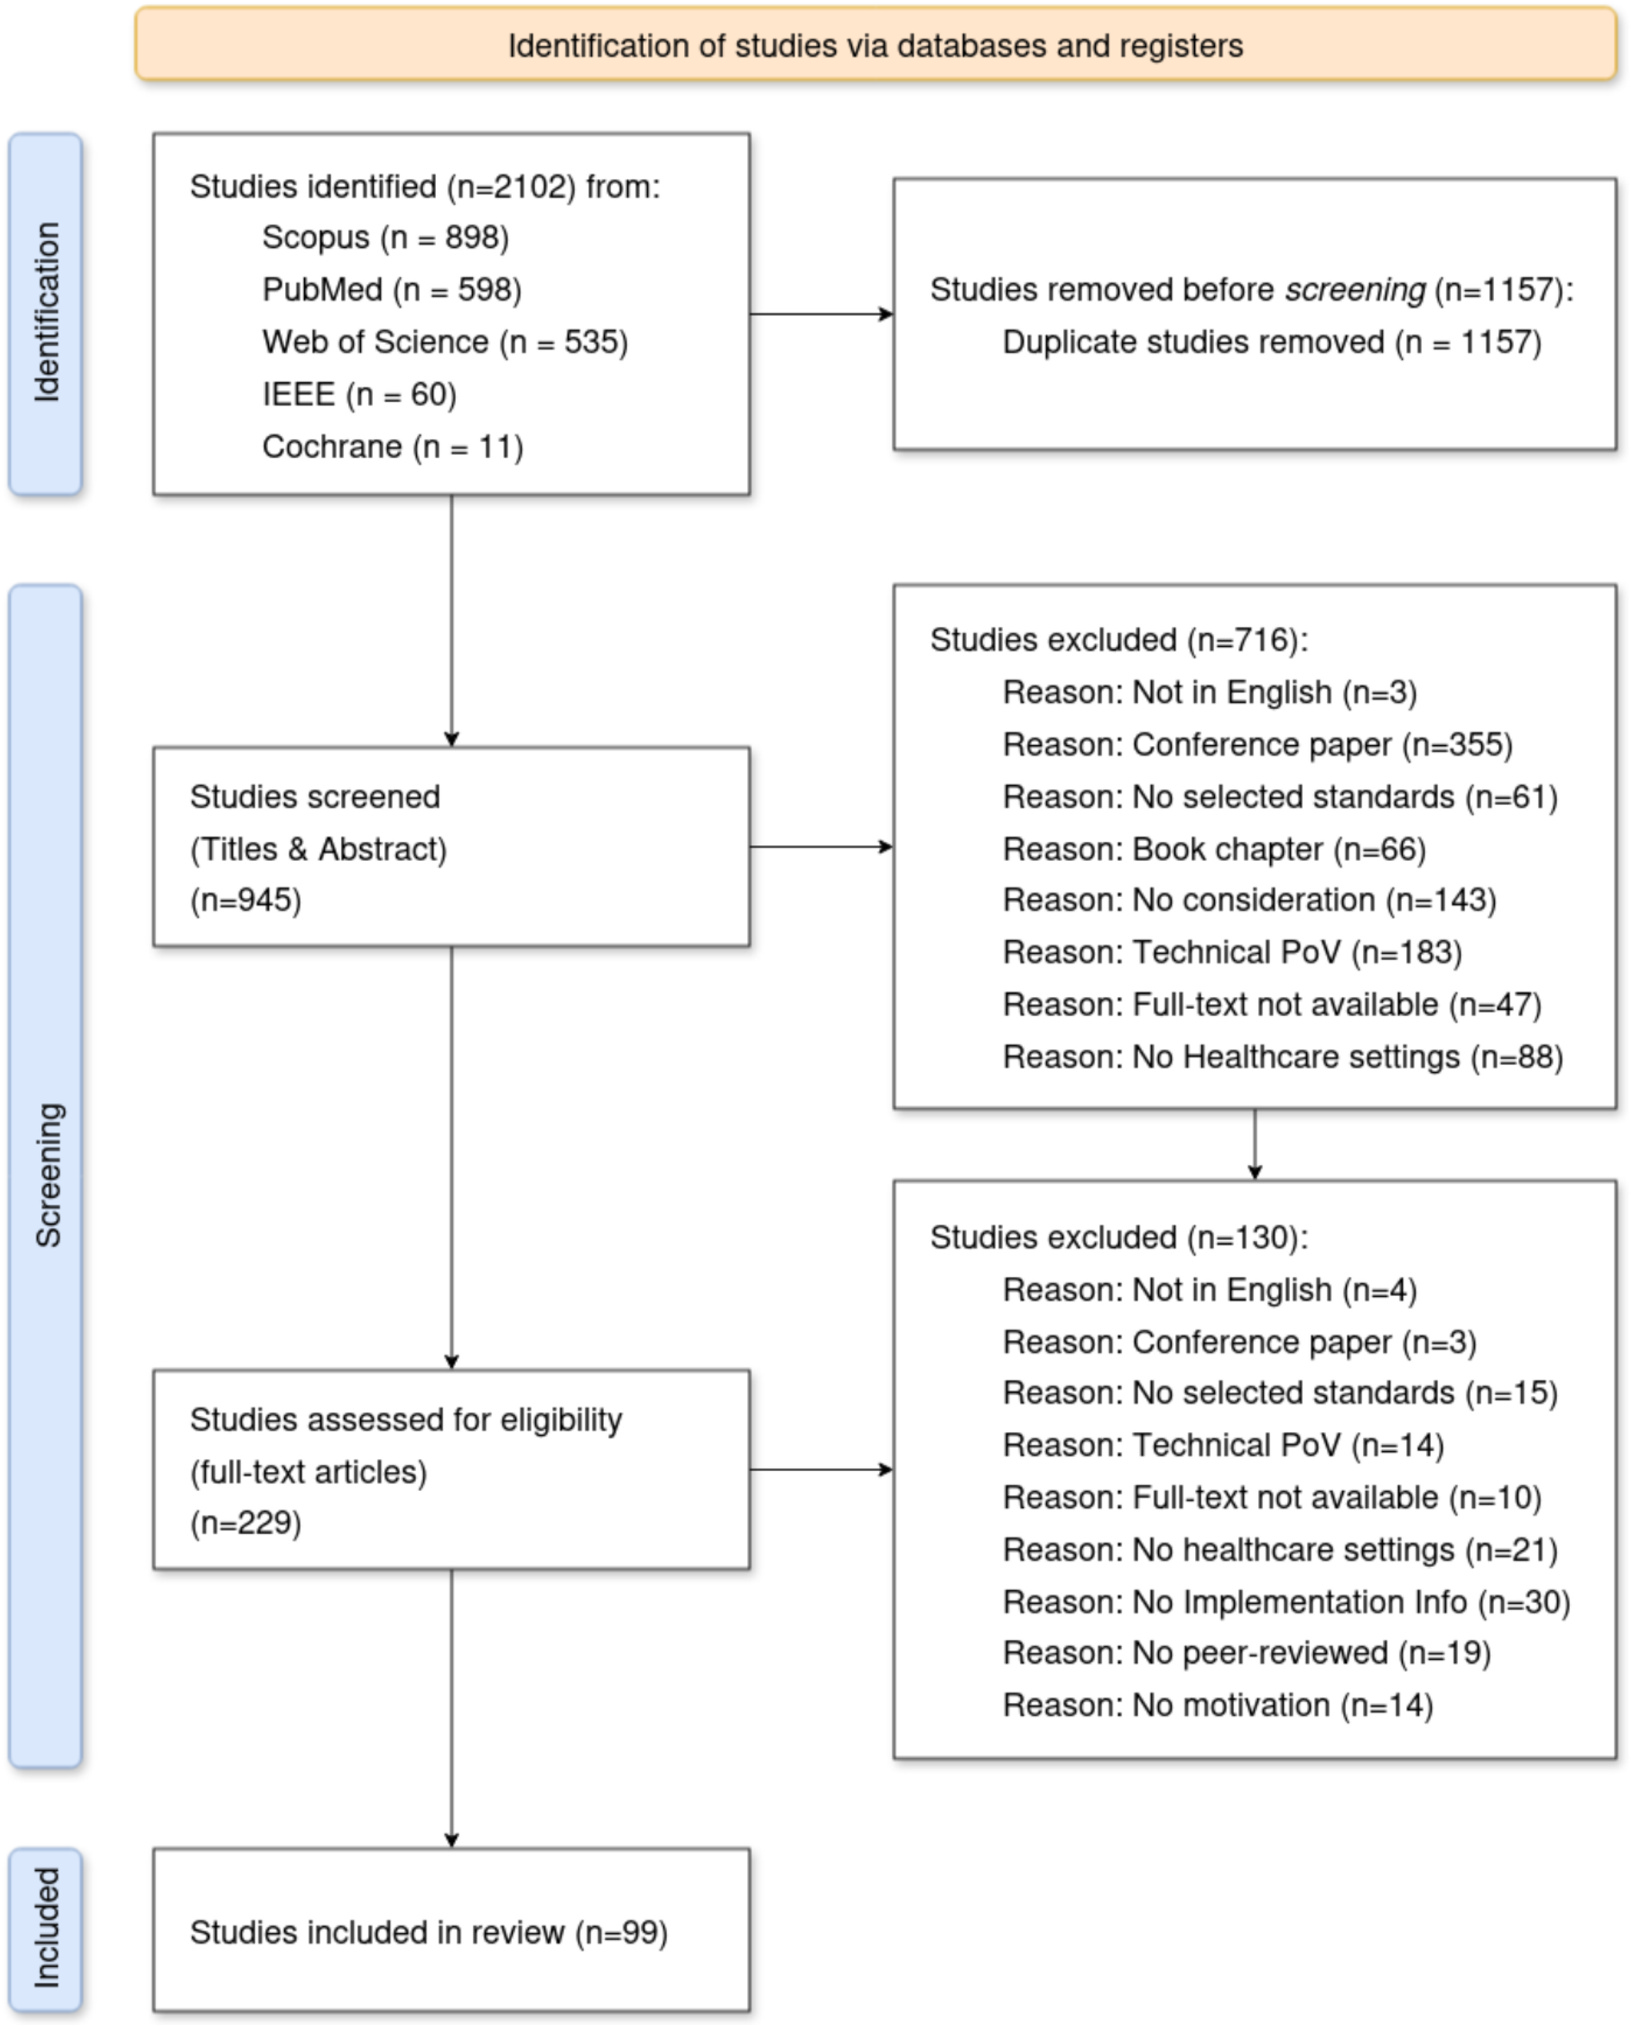
\includegraphics[width=\textwidth]{figures/paper1/fig1-prisma.jpg}
\caption{PRISMA flow diagram illustrating the study selection process, including identification, screening, eligibility assessment, and final inclusion of studies.}
\label{fig:paper1_prisma}
\end{figure}

\subsubsection{Inclusion criteria}
\label{sec:paper1_inclusion_criteria}

The inclusion criteria were as follows: the full text of the article had to be accessible, and the article needed to be available in English. Only studies published in peer-reviewed journals between 2021 and 2024 were considered. The review was limited to peer-reviewed scientific publications to ensure methodological transparency and reproducibility; grey literature and unpublished sources were excluded due to the lack of standardized appraisal frameworks and potential bias.

Eligible studies were required to report on FHIR, OMOP-CDM, or openEHR, to adopt the data standards in real-world or real-like healthcare settings, to discuss the standards from a technical perspective while also considering their practical or organizational aspects for a real-world application, to offer motivation for the use of the selected standards, and to detail how health data standards were adopted, including tools and methods used. The review was intentionally limited to these three standards, as they represent the leading open, community-driven, and freely available health data frameworks, each addressing complementary phases of the data lifecycle \cite{tsafnat_converge_2024}.

We selected 2021 as the starting date for this review as this overlaps with the COVID-19 pandemic, which significantly accelerated the adoption of digital tools. This shift, driven by the urgent need to maintain high-quality healthcare services, was observed both across the European Union and globally \cite{noauthor_repowereu_2022}.

% Paper 1, Table 1 -- transcribed from the published PDF (row order and cell contents as in the PDF text layer).
% Cell text that the PDF continued across a page break has been re-attached to its row (see integration report).
% Layout only: wider margins on the landscape pages of this 99-row table (rows cannot break across pages).
\newgeometry{margin=2cm}
\begin{landscape}
\scriptsize
\setlength{\tabcolsep}{2pt}
\begin{longtable}{>{\raggedright\arraybackslash}p{2.0cm} >{\raggedright\arraybackslash}p{3.8cm} >{\raggedright\arraybackslash}p{1.7cm} >{\raggedright\arraybackslash}p{1.5cm} >{\raggedright\arraybackslash}p{1.3cm} >{\raggedright\arraybackslash}p{7.4cm} >{\raggedright\arraybackslash}p{1.8cm} >{\raggedright\arraybackslash}p{1.3cm} >{\raggedright\arraybackslash}p{1.9cm} >{\raggedright\arraybackslash}p{1.4cm}}
\caption{Summary of extracted data from selected studies, including key characteristics, major application domains, and reported challenges.}
\label{tab:paper1_summary}\\
\toprule
\multicolumn{1}{l}{\textbf{Ref}} & \textbf{Title} & \textbf{Study Location} & \textbf{Health Data Standard} & \textbf{Scale} &
\multicolumn{2}{l}{\textbf{Objective for using the standard}} & \multicolumn{3}{l}{\textbf{Application domain}} \\
 & & & & & \textbf{Detailed} & \textbf{Category} & \textbf{Type} & \textbf{Healthcare Area} & \textbf{Use} \\
\midrule
\endfirsthead
\multicolumn{10}{l}{Table~\ref{tab:paper1_summary} (continued)}\\
\midrule
\multicolumn{1}{l}{\textbf{Ref}} & \textbf{Title} & \textbf{Study Location} & \textbf{Health Data Standard} & \textbf{Scale} &
\multicolumn{2}{l}{\textbf{Objective for using the standard}} & \multicolumn{3}{l}{\textbf{Application domain}} \\
 & & & & & \textbf{Detailed} & \textbf{Category} & \textbf{Type} & \textbf{Healthcare Area} & \textbf{Use} \\
\midrule
\endhead
\midrule
\multicolumn{10}{r}{(continued on next page)}\\
\endfoot
\bottomrule
\endlastfoot
Baumgartner et al., 2024 & Health data space nodes for privacy-preserving linkage of medical data to support collaborative secondary analyses & Austria & OMOP-CDM & National & The primary objective of this study is to propose and evaluate a federated, node-based system architecture called Health Data Space (HDS) nodes to enhance decentralized health data management and analytics. Harmonize heterogeneous data into the OMOP-CDM, which is well-suited for observational health data. & Data Reuse & Research & Clinical Medicine & Secondary \\
Bhattacharjee et al., 2024 & INSPIRE datahub: a pan-African integrated suite of services for harmonising longitudinal population health data using OHDSI tools & Kenya; South Africa; Tanzania & OMOP-CDM & Multi Center & This paper introduces the INSPIRE datahub as a comprehensive solution for data integration and harmonization. Functioning as a pan-African, federated research ecosystem, the datahub is designed to adhere to the principles of FAIR. It tackles critical issues related to reproducibility, standardization, and scalability of data harmonization and sharing systems, primarily in low-resource settings, leveraging existing technologies customized for optimal use. & Data Reuse & Research & Public Health & Secondary \\
Phelan et al., 2024 & Beyond compliance with the 21st Century Cures Act Rule: a patient controlled electronic health information export application programming interface & USA & FHIR & National & The authors formulate a model for interoperable, patient-controlled, app-driven access to EHI exports in an open-source reference implementation following the Argonaut FHIR Accelerator consensus implementation guide for EHI Export. & Data Exchange & Research & Public Health & Secondary \\
Shehab et al., 2024 & The National Healthcare Safety Network's digital quality measures: CDC's automated measures for surveillance of patient safety & USA & FHIR & National & The article outlines NHSN's use of NHSNLink and FHIR APIs to automate public health surveillance via digital quality measures (dQMs), focusing on preventable patient harms like hypoglycemia, C. difficile infection, and venous thromboembolism, piloted through the NHSNCoLab program. & Data Exchange & Clinical & Public Health & Secondary \\
Ulgu et al., 2024 & A Nationwide Chronic Disease Management Solution via Clinical Decision Support Services: Software Development and Real-Life Implementation Report & Turkey & FHIR & National & The DMP (Disease Management Platform) aims to enhance data interoperability with Turkey's central national EHR (e-Nabiz) using HL7 FHIR, allowing data sharing and supporting the screening and monitoring for chronic diseases at the national level. & CDS & Clinical & Clinical Medicine & Secondary \\
Ward et al., 2024 & The OMOP common data model in Australian primary care data: Building a quality research ready harmonised dataset & Australia & OMOP-CDM & National & In this research, the authors aim to investigate the use of the open-source OMOP-CDM in the PATRON primary care data repository. & Data Reuse & Research & Public Health & Secondary \\
Bennett et al., 2023 & MIMIC-IV on FHIR: converting a decade of in-patient data into an exchangeable, interoperable format & Germany; Canada; Netherlands & FHIR & Multi Center & To convert the MIMIC-IV database into FHIR. Additionally, generate and publish an openly available demo of the resources, and create a FHIR Implementation Guide to support and clarify the usage of MIMIC-IV on FHIR. & Data Reuse & Research & Public Health & Secondary \\
Cai et al., 2023 & Advancing Toward a Common Data Model in Ophthalmology & USA & OMOP-CDM & Single Center & To identify gaps in OMOP concept coverage to enhance the standard's ability to accommodate ophthalmology concepts for vision research. & Vocabulary definition & Research & Clinical Services and Diagnostics & Secondary \\
Carus et al., 2023 & Mapping the Oncological Basis Dataset to the Standardized Vocabularies of a Common Data Model: A Feasibility Study & Germany & OMOP-CDM & National & The authors mapped oncological basis dataset (oBDS) elements to the standardized vocabularies, a metadata repository of the observational medical outcomes partnership (OMOP) common data model (CDM). & Data Reuse & Research & Clinical Medicine & Secondary \\
Chechulina et al., 2023 & Semi-Automated Mapping of German Study Data Concepts to an English Common Data Model & Germany & OMOP-CDM & Single Center & To establish a mapping approach that automatically translates German data variable names into English and suggests OMOP concepts. The study focuses on improving the process of mapping medical data from the Hamburg City Health Study (HCHS) to the OMOP-CDM. & Data Reuse & Research & Clinical Medicine & Secondary \\
Mayer et al., 2023 & Learning important common data elements from shared study data: The All of Us program analysis & USA & OMOP-CDM & National & The study aims at gathering different datasets involved in the same national program to identify the common and unique elements within each dataset to guide future study design. & Data Reuse & Research & Public Health & Secondary \\
Dolin et al., 2023 & Sync for Genes Phase 5: Computable artifacts for sharing dynamically annotated FHIR-formatted genomic variants & USA & FHIR & Single Center & The objective of the study is to standardize the sharing of dynamically annotated genetic variants, enabling clinical decision support applications to provide up-to-date, real-time genomic annotations for clinical decision-making. & CDS & Research & Biomedical Sciences & Secondary \\
Einsestein et al., 2023 & Economic Analysis of a Single Institutional Review Board Data Exchange Standard in Multisite Clinical Studies & USA & FHIR & / & The authors conducted a study to determine whether the use of this standard would be economically attractive for sIRB workflows collectively and for Reviewing and Relying institutions. & Data Exchange & Research & Health Information Management & Secondary \\
Espinoza et al., 2023 & Development of an OpenMRS-OMOP ETL tool to support informatics research and collaboration in LMICs & USA & OMOP-CDM & Single Center & To develop a free, open-source ETL pipeline to transform clinical data in OpenMRS instances into OMOP. & Data Reuse & Research & Clinical Medicine & Secondary \\
Guo et al., 2023 & Development and validation of the SickKids Enterprise-wide Data in Azure Repository (SEDAR) & Canada & OMOP-CDM & Single Center & To describe the processes developed by The Hospital for Sick Children (SickKids) to enable utilization of electronic health record (EHR) data by creating sequentially transformed schemas for use across multiple user types. Enable multicenter research and machine learning by adopting the OMOP Common Data Model (CDM), & Data Reuse & Research & Clinical Medicine & Secondary \\
Henke et al., 2023 & Assessing the Use of German Claims Data Vocabularies for Research in the Observational Medical Outcomes Partnership Common Data Model: Development and Evaluation Study & Germany & OMOP-CDM & Multi Center & This study aims to increase the coverage of German vocabularies in the OMOP CDM. & Vocabulary definition & Research & Health Information Management & Secondary \\
Jones et al., 2023 & Real World Performance of the 21st Century Cures Act Population Level Application Programming Interface & USA & FHIR & Multi Center & To evaluate the real-world performance in delivering patient data on populations of the SMART/HL7 Bulk FHIR Access API, required in Electronic Health Records (EHRs) under the 21st Century Cures Act Rule. & Data Exchange & Research & Public Health & Secondary \\
Kempf et al., 2023 & How to Improve Cancer Patients ENrollment in Clinical Trials From rEal-Life Databases Using the Observational Medical Outcomes Partnership Oncology Extension: Results of the PENELOPE Initiative in Urologic Cancers & France & OMOP-CDM & Single Center & The authors wanted to assess the added value of the Oncology Extension of the Observational Medical Outcomes Partnership (OMOP) common data model (CDM) to automatically identify patients with cancer for inclusion in clinical trials (CTs). & CDS & Research & Clinical Medicine & Secondary \\
Kim et al., 2023 & Scalable Infrastructure Supporting Reproducible Nationwide Healthcare Data Analysis toward FAIR Stewardship & South Korea & OMOP-CDM & National & To standardize the national claims data from the HIRA Service of South Korea into the OMOP-CDM, and to build a scalable infrastructure providing accessible and flexible data analysis environments with privacy-by-design protection. & Data Exchange & Research & Health Information Management & Secondary \\
Kiwuwa-Muyingo et al., 2023 & Enabling data sharing and utilization for African population health data using OHDSI tools with an OMOP-common data model & Sub-Saharan Africa & OMOP-CDM & Multi Center & To describe the INSPIRE initiative's innovative approach to data sharing and its efforts to build a FAIR, borderless population health research platform. The paper outlines how this platform leverages OMOP-CDM to facilitate longitudinal population health research and clinical research, with an emphasis on addressing challenges in data sharing within the context of Sub-Saharan Africa (SSA). & CDS & Research & Biomedical Sciences & Secondary \\
Kohler et al., 2023 & Eos and OMOCL: Towards a seamless integration of openEHR records into the OMOP Common Data Model & Germany & OMOP-CDM; openEHR & Multi Center & Both Eos and OMOCL provide a way to define generic mappings for the integration of openEHR records into OMOP. & Data Reuse & Research & Biomedical Sciences & Secondary \\
Mayer, 2023 & Conversion of CPRD AURUM data into the OMOP common data model & UK & OMOP-CDM & National & The author's objective was to convert a static copy of CPRD AURUM data into the OMOP CDM and run existing tools on the converted data. & Data Reuse & Research & Public Health & Secondary \\
Oja et al., 2023 & Transforming Estonian health data to the Observational Medical Outcomes Partnership (OMOP) Common Data Model: Lessons learned & Estonia & OMOP-CDM & National & To describe the reusable process of electronic health records (EHR), claims, and prescriptions data into Observational Medical Outcome Partnership (OMOP) Common Data Model (CDM), together with challenges faced and solutions implemented. & Data Reuse & Research & Health Information Management & Secondary \\
Oliver et al., 2023 & Introducing the BlendedICU dataset, the first harmonized, international intensive care dataset & France & OMOP-CDM & Multi Center & This study introduces the BlendedICU dataset, a massive dataset of international intensive care data. This dataset aims to facilitate generalizability studies of machine learning models, as well as statistical studies of clinical practices in intensive care units. & Data Reuse & Research & Clinical Services and Diagnostics & Secondary \\
Park et al., 2023 & Cancer Research Line (CAREL): Development of Expanded Distributed Research Networks for Prostate Cancer and Lung Cancer & South Korea & OMOP-CDM & Multi Center & The authors attempted to develop DRNs (Distributed Research Networks) for multicenter research that can be easily installed and used by any institution. & Data Reuse & Research & Clinical Medicine & Secondary \\
Peng et al., 2023 & An ETL-process design for data harmonization to participate in international research with German real-world data based on FHIR and OMOP CDM & Germany & FHIR; OMOP-CDM & National & To develop an ETL process that enables German university hospitals to participate in international networks, such as the DARWIN EU project, by: 1. Transforming German patient data from HL7 FHIR to OMOP CDM. 2. Processing large volumes of data efficiently. 3. Ensuring flexibility to accommodate changes in FHIR profiles. & Data Reuse & Research & Public Health & Secondary \\
Rinaldi et al., 2023 & Towards interoperability in infection control: a standard data model for microbiology & Germany & FHIR & National & The objective was to develop a dataset definition, information model, and FHIR® specification for key data elements contained in a German molecular genomics (MolGen) report to facilitate genomic and phenotype integration in electronic health records. & Vocabulary definition & Research & Clinical Medicine & Secondary \\
Raventós et al., 2023 & Transforming the Information System for Research in Primary Care (SIDIAP) in Catalonia to the OMOP Common Data Model and Its Use for COVID-19 Research & Spain & OMOP-CDM & Regional & The primary aim of this work was to convert the Information System for Research in Primary Care (SIDIAP) from Catalonia, Spain, to the Observational Medical Outcomes Partnership (OMOP) Common Data Model (CDM). & Data Reuse & Research & Biomedical Sciences & Secondary \\
Rinaldi et al., 2023 & Towards interoperability in infection control: a standard data model for microbiology & Germany & FHIR & National & The goal is to offer one common format for microbiology data that can be publicly adopted across different institutions and to provide a common international terminology in place of, or together with, the local codes to enhance interoperability. & Vocabulary definition & Research & Clinical Services and Diagnostics & Secondary \\
Sadsad et al., 2023 & A computable biomedical knowledge object for calculating in-hospital mortality for patients admitted with acute myocardial infarction & Australia & OMOP-CDM & National & To calculate in-hospital mortality of patients admitted for acute myocardial infarction (AMI). & CDS & Research & Clinical Medicine & Secondary \\
Seol et al., 2023 & Effect of statin use on head and neck cancer prognosis in a multicenter study using a Common Data Model & South Korea & OMOP-CDM & Multi Center & The authors examined the effect of statin use on HNC recurrence using the converted OMOP-CDM in seven hospitals between 1986 and 2022. & CDS & Research & Clinical Medicine & Secondary \\
Sinaci et al., 2023 & A Data Transformation Methodology to Create Findable, Accessible, Interoperable, and Reusable Health Data: Software Design, Development, and Evaluation Study & Spain & FHIR & Multi Center & To create a methodology for ETL health data into HL7 FHIR repositories following FAIR principles and develop a Data Curation Tool to apply it. & Data Reuse & Research & Public Health & Secondary \\
Song et al., 2023 & Implementation of a Patient Summary Web Application According to the International Patient Summary and Validation in Common Use Cases in Japan & Japan & FHIR & Single Center & This study aimed to develop a patient summary application that summarizes and visualizes patient information accumulated by existing systems. & Data Exchange; Data Reuse & Clinical & Public Health & Primary \\
Tang et al., 2023 & Creating a Medical Imaging Workflow Based on FHIR, DICOMweb, and SVG & Taiwan & FHIR & / & In this study, the authors developed a demonstration system in which FHIR and DICOMweb specifications are used to facilitate the integration of conventional HIS (Hospital Information System) and PACS (Picture Archiving and Communication System). & Data Exchange & Research & Clinical Services and Diagnostics & / \\
Yu et al., 2023 & Integrating real-world data to assess cardiac ablation device outcomes in a multicenter study using the OMOP common data model for regulatory decisions: implementation and evaluation & USA & OMOP-CDM & Multi Center & Describe the application of the Observational Medical Outcomes Partnership (OMOP) common data model (CDM) for supporting medical device real-world evaluation in a National Evaluation System for health Technology Coordinating Center (NESTcc) Test-Case involving two healthcare systems, Mercy Health and Mayo Clinic. & Data Reuse & Research & Clinical Medicine & Secondary \\
Almeida et al., 2022 & BIcenter-AD: Harmonising Alzheimer's Disease cohorts using a common ETL tool & Portugal & OMOP-CDM & Multi Center & The manuscript proposes a collaborative ETL tool designed to harmonize data sources in multi-institutional environments. & Data Reuse & Research & Clinical Medicine & Secondary \\
Bae et al., 2022 & Development of eClaim system for private indemnity health insurance in South Korea: Compatibility and interoperability & South Korea & FHIR & National & This study developed an FHIR®-based electronic claim (eClaim) service to address issues with paper-based workflows, ensuring usability, accessibility, and compatibility with legacy systems. The eClaim service for PIHI has been operational since 2017. & Data Exchange & Clinical & Health Information Management & Primary \\
Bae et al., 2022 & Coronary Artery Computed Tomography Angiography for Preventing Cardio-Cerebrovascular Disease: Observational Cohort Study Using the Observational Health Data Sciences and Informatics' Common Data Model & South Korea & OMOP-CDM & Single Center & The objective of the study was to investigate the effectiveness of Coronary artery computed tomography angiography (CCTA) screening on Cardio-cerebrovascular diseases (CVDs) outcomes by using the OMOP-CDM data and the population-level estimation method. & CDS & Research & Clinical Medicine & Secondary \\
Bathelt et al., 2022 & Opportunities of Digital Infrastructures for Disease Management---Exemplified on COVID-19-Related Change in Diagnosis Counts for Diabetes-Related Eye Diseases & Germany & OMOP-CDM & Multi Center & To demonstrate (1) how to facilitate digital infrastructures to run a retrospective study in a research network spread across university and non-university hospital sites; and (2) to answer a medical question on COVID-19 related change in diagnostic counts for diabetes-related eye diseases. & Data Reuse & Research & Biomedical Sciences & Secondary \\
Bialke et al., 2022 & A FHIR has been lit on gICS: facilitating the standardised exchange of informed consent in a large network of university medicine & Germany & FHIR & Multi Center & To implement a standardized solution for the FHIR-compliant provision of consent information using gICS. & Data Exchange & Research & Health Information Management & Secondary \\
Bradshaw et al., 2022 & GARDE: a standards-based clinical decision support platform for identifying population health management cohorts & USA & FHIR & Multi Center & To design and implement a scalable standards-based clinical decision support (CDS) approach to identify patient cohorts for PHM and maximize opportunities for multi-site dissemination. & CDS & Clinical & Clinical Medicine & Primary \\
Byun et al., 2022 & Analysis of treatment pattern of anti-dementia medications in newly diagnosed Alzheimer's dementia using OMOP CDM & Korea & OMOP-CDM & Multi Center & OMOP CDM was used for standardized, large-scale, multi-center analysis of AD treatment. & CDS & Research & Clinical Medicine & Secondary \\
Carus et al., 2022 & Mapping Cancer Registry Data to the Episode Domain of the Observational Medical Outcomes Partnership Model (OMOP) & Germany & OMOP-CDM & National & The objective of this study was firstly to find out to what extent the source terminologies of the clinical cancer registry can be mapped to the respective OMOP standard. & Vocabulary definition & Research & Clinical Medicine & Secondary \\
Castano et al., 2022 & Identification of patients with drug-resistant epilepsy in electronic medical record data using the Observational Medical Outcomes Partnership Common Data Model & USA & OMOP-CDM & Single Center & The authors aim to develop and compare the performance of computable phenotypes for drug-resistant epilepsy (DRE) using the OMOP Common Data Model. & CDS & Research & Clinical Medicine & Secondary \\
Choi et al., 2022 & Conversion of Automated 12-Lead Electrocardiogram Interpretations to OMOP CDM Vocabulary & South Korea & OMOP-CDM & Multi Center & The authors aim to develop a fully automated text data conversion algorithm that overcomes the limitations of existing tools and manual conversion. & Data Reuse; Vocabulary definition & Research & Clinical Medicine & Secondary \\
Chukwu et al., 2022 & Standardizing Primary Health Care Referral Data Sets in Nigeria: Practitioners' Survey, Form Reviews, and Profiling of Fast Healthcare Interoperability Resources (FHIR) & Nigeria & FHIR & Regional & The objective of this study is to design FHIR profiles and present methodology and the profiled FHIR resource for Maternal and Child Health referral use cases in Ebonyi state, Nigeria---a typical low- and middle-income country (LMIC) setting. & Vocabulary definition & Research & Clinical Medicine & Secondary \\
Delanerolle et al., 2022 & Methodological Issues in Using a Common Data Model of COVID-19 Vaccine Uptake and Important Adverse Events of Interest: Feasibility Study of Data and Connectivity COVID-19 Vaccines Pharmacovigilance in the United Kingdom & UK & OMOP-CDM & National & This study aims to use the concept mappings in the OMOP-CDM to identify common concepts recorded and to report these in a repeated cross-sectional study. & Data Reuse & Research & Biomedical Sciences & Secondary \\
Gruendner et al., 2022 & The Architecture of a Feasibility Query Portal for Distributed COVID-19 Fast Healthcare Interoperability Resources (FHIR) Patient Data Repositories: Design and Implementation Study & Germany & FHIR & National & This study described the design and implementation of the components involved in creating a cross-hospital feasibility query platform for researchers based on FHIR resources. This effort was part of a large COVID-19 data exchange platform and was designed to be scalable for a broad range of patient data. & CDS;Data Exchange & Research & Biomedical Sciences & Secondary \\
Jung et al., 2022 & Patient-Level Fall Risk Prediction Using the Observational Medical Outcomes Partnership's Common Data Model: Pilot Feasibility Study & South Korea & OMOP-CDM & Single Center & The objectives of this study were to (1) convert fall-related electronic health record data into OMOP common data model format and (2) develop models that predict fall risk during 2 time periods. & CDS & Research & Clinical Medicine & Secondary \\
Jung et al., 2022 & Shared Interoperable Clinical Decision Support Service for Drug-Allergy Interaction Checks: Implementation Study & South Korea & FHIR & National & The study focuses on developing and deploying the national CDS service for drug-allergy interaction (DAI) to check for healthcare providers in Korea which need to introduce the service but lack the budget and expertise. & CDS;Data Exchange & Clinical & Clinical Services and Diagnostics & Secondary \\
Junior et al., 2022 & Integrating real-world data from Brazil and Pakistan into the OMOP common data model and standardized health analytics framework to characterize COVID-19 in the Global South & Pakistan; Brazil & OMOP-CDM & Multi Center & This work aims to demonstrate the use of a standardized health informatics framework to generate reliable and reproducible real-world evidence from Latin America and South Asia towards characterizing coronavirus disease 2019 (COVID-19) in the Global South. & Data Reuse & Research & Biomedical Sciences & Secondary \\
K Sommer et al., 2022 & Structured, Harmonized, and Interoperable Integration of Clinical Routine Data to Compute Heart Failure Risk Scores & Germany & openEHR & Multi Center & To demonstrate the feasibility of deriving and calculating heart failure (HF) risk scores (MAGGIC and Barcelona Bio-HF) from clinical routine data using an interoperable, harmonized core dataset within the openEHR framework. & CDS & Research & Clinical Medicine & Secondary \\
Lazarova et al., 2022 & An Interoperable Electronic Health Record System for Clinical Cardiology & Italy & FHIR & Regional & The main aim of the project is to design, produce, deploy, and test a new modular electronic health record system (EHRS) to be used in the cardiological wards of some local hospitals. The main objective has been to replace the paper-based system. & Data Exchange; EHR Design & Clinical & Clinical Medicine & Primary \\
Li et al., 2022 & A configurable method for clinical quality measurement through electronic health records based on openEHR and CQL & China & openEHR & Single Center & To help clinical staff develop clinical quality indicators to monitor and improve the performance and quality of healthcare services. & CDS & Clinical & Clinical Medicine & Secondary \\
McGuinness et al., 2022 & Extraction of Electronic Health Record Data using Fast Healthcare Interoperability Resources for Automated Breast Cancer Risk Assessment & USA & FHIR & Single Center & To discuss the development of web-based tools for breast cancer risk assessment, barriers to their use, and the potential for automating risk calculations using FHIR to improve patient care and decision-making. & CDS & Research & Clinical Medicine & Secondary \\
Papez et al., 2022 & Transforming and evaluating electronic health record disease phenotyping algorithms using the OMOP common data model: a case study in heart failure & UK & OMOP-CDM & Multi Center & The authors' objective was to convert the UK Biobank, a study of 500 000 participants with rich genetic and phenotypic data to the Observational Medical Outcomes Partnership (OMOP) CDM. & Data Reuse & Research & Public Health & Secondary \\
Phuong et al., 2022 & Extracting Patient-level Social Determinants of Health into the OMOP Common Data Model & USA & OMOP-CDM & Multi Center & This paper uses the University of Washington Enterprise Data Warehouse (a data contributor to N3C) to demonstrate how SDoH can be represented and managed to be made available within an OMOP common data model. & Data Reuse & Research & Biomedical Sciences & Secondary \\
Román-Villarán et al., 2022 & A Personalized Ontology-Based Decision Support System for Complex Chronic Patients: Retrospective Observational Study & Spain & FHIR & Multi Center & To design, develop, and validate an ontology-based CDSS that provides personalized recommendations related to drug prescription. & CDS & Research & Clinical Medicine & Secondary \\
Rosenau et al., 2022 & Generation of a Fast Healthcare Interoperability Resources (FHIR)-based Ontology for Federated Feasibility Queries in the Context of COVID-19: Feasibility Study & Germany & FHIR & National & This study investigates how search ontology can be automatically generated using FHIR profiles and a terminology server. Furthermore, it describes how this ontology can be used in a user interface (UI) and how a mapping and a terminology tree created together with the ontology can translate user input into FHIR queries. & Vocabulary definition & Research & Biomedical Sciences & Secondary \\
Spotnitz et al., 2022 & Patient characteristics and antiseizure medication pathways in newly diagnosed epilepsy: Feasibility and pilot results using the common data model in a single-center electronic medical record database & USA & OMOP-CDM & Single Center & To demonstrate the feasibility of characterizing adult patients with epilepsy and ASM treatment pathways using the CDM in an electronic health record (EHR)-derived database. & CDS & Research & Clinical Medicine & Secondary \\
Wang et al., 2022 & The sociodemographic characteristics and clinical features of the late-life depression patients: results from the Beijing Anding Hospital mental health big data platform & China & OMOP-CDM & Single Center & This study aimed to explore the psychiatric outpatient attendance of LLD (late-life depression) patients at a psychiatric hospital in China, with a subgroup analysis, such as with or without anxiety, gender differences. & CDS & Research & Clinical Medicine & Secondary \\
Xing Tan et al., 2022 & Applying the OMOP Common Data Model to Facilitate Benefit-Risk Assessments of Medicinal Products Using Real-World Data from Singapore and South Korea & Singapore; South Korea & OMOP-CDM & Multi Center & The aim of this study was to characterize the potential usefulness of CDM conversion by conducting a sample benefit-risk assessment involving CDM-converted data. & CDS; Data Reuse & Research & Clinical Medicine & Secondary \\
Yoo et al., 2022 & Transforming Thyroid Cancer Diagnosis and Staging Information from Unstructured Reports to the Observational Medical Outcome Partnership Common Data Model & South Korea & OMOP-CDM & Multi Center & The authors aimed to demonstrate the applicability of the OMOP CDM oncology extension module for thyroid cancer diagnosis and cancer stage information by processing free-text medical reports. & Data Reuse & Research & Clinical Medicine & Secondary \\
Yu et al., 2022 & Developing an ETL tool for converting the PCORnet CDM into the OMOP CDM to facilitate the COVID-19 data integration & USA & OMOP-CDM & Single Center & The objective of this study is to design, develop, and evaluate an ETL tool that transforms the PCORnet CDM format data into the OMOP CDM. & Data Reuse & Research & Biomedical Sciences & Secondary \\
Almeida et al., 2021 & A methodology for cohort harmonisation in multicentre clinical research & Portugal & OMOP-CDM & Multi Center & To present a methodology to extract relevant concepts from clinical notes to enrich structured OMOP CDM databases, enabling the use of SQL queries for analyzing clinical text information. & Data Reuse & Research & Clinical Services and Diagnostics & Secondary \\
Almeida et al., 2021 & A two-stage workflow to extract and harmonize drug mentions from clinical notes into observational databases & Germany; Netherlands & OMOP-CDM & Multi Center & To harmonize different cohorts into a standard data schema, facilitating multi-cohort querying and analysis. & Data Reuse; Data Exchange & Research & Clinical Medicine & Secondary \\
Biedermann et al., 2021 & Standardizing registry data to the OMOP Common Data Model: experience from three pulmonary hypertension databases & USA;Europe and Canada & OMOP-CDM & Multi Center & The study objective is to document the process and outcomes of transforming registry data in PH (Pulmonary Hypertension) to the OMOP CDM, highlighting challenges and providing potential solutions. & Data Reuse & Research & Clinical Medicine & Secondary \\
Carvalho Gomes et al., 2021 & Representation of Diagnosis and Nursing Interventions in OpenEHR Archetypes & Brazil & openEHR & Single Center & The study aimed to represent the content of nursing diagnosis and interventions in the openEHR standard. & EHR Design & Research & Clinical Services and Diagnostics & Secondary \\
De et al., 2021 & Analyzing Patient Secure Messages Using a Fast Health Care Interoperability Resources (FIHR)-Based Data Model: Development and Topic Modeling Study & USA & FHIR & Single Center & To develop a data model for patient secure messages based on the FHIR standard to extract significant information. & Vocabulary definition & Research & Public Health & Secondary \\
Dolin et al., 2021 & Sync for Genes Phase 5: Computable artifacts for sharing dynamically annotated FHIR-formatted genomic variants & USA & FHIR & National & To describe an open-source utility for converting variants from VCF format into HL7 FHIR format & Data Exchange & Research & Biomedical Sciences & Secondary \\
González-Castro et al., 2021 & CASIDE: A data model for interoperable cancer survivorship information based on FHIR & Spain & FHIR & Multi Center & To present CASIDE, an interoperable data model for cancer survivorship information that aims to accelerate the secondary use of healthcare data and data sharing across institutions. It is designed to provide a holistic view of the cancer survivor, taking into account not just the clinical data but also the patient's own perspective, and is built upon the emerging FHIR standard. & Data Reuse; Vocabulary definition & Research & Clinical Medicine & Secondary \\
Gruendner et al., 2021 & The Architecture of a Feasibility Query Portal for Distributed COVID-19 Fast Healthcare Interoperability Resources (FHIR) Patient Data Repositories: Design and Implementation Study & Germany & FHIR & Single Center & To elucidate how FHIR data can be queried directly with a preprocessing service and be used for statistical analyses. & Data Reuse & Research & Public Health & Secondary \\
Guinez-Molinos et al., 2021 & Interoperable Platform to Report Polymerase Chain Reaction SARS-CoV-2 Tests From Laboratories to the Chilean Government: Development and Implementation Study & Chile & FHIR & Single Center & This study aims to design and develop an interoperable platform to report polymerase chain reaction (PCR) SARS-CoV-2 tests from laboratories to the Chilean government. & Data Exchange & Clinical & Biomedical Sciences & Secondary \\
Gulden et al., 2021 & Prototypical Clinical Trial Registry Based on Fast Healthcare Interoperability Resources (FHIR): Design and Implementation Study & Germany & FHIR & Multi Center & This study investigates how Health Level 7 (HL7) Fast Healthcare Interoperability Resources (FHIR) may be used as a standardized format for exchanging and storing clinical trial records. & Data Exchange & Research & Health Information Management & Secondary \\
Kawamoto et al., 2021 & Establishing a multidisciplinary initiative for interoperable electronic health record innovations at an academic medical center & USA & FHIR & Multi Center & To establish an enterprise initiative for improving health and health care through interoperable electronic health record (EHR) innovations. & EHR Design & Clinical & Public Health & Primary \\
Khalifa et al., 2021 & Interoperable genetic lab test reports: mapping key data elements to HL7 FHIR specifications and professional reporting guidelines & USA & FHIR & Single Center & This study aims to identify various data content of some genetic lab test reports and map them to FHIR CG IG specifications to assess its coverage and to provide some suggestions for standard development and implementation. & Vocabulary definition & Research & Biomedical Sciences & Secondary \\
Kim et al., 2021 & Transforming electronic health record polysomnographic data into the Observational Medical Outcome Partnership's Common Data Model: a pilot feasibility study & South Korea & OMOP-CDM & Multi Center & The study aimed to assess the link between irritable bowel syndrome (IBS) medications and the risk of osteoporosis and fractures. & CDS & Research & Clinical Medicine & Secondary \\
Kim et al., 2021 & The Risk of Osteoporosis and Osteoporotic Fracture Following the Use of Irritable Bowel Syndrome Medical Treatment: An Analysis Using the OMOP CDM Database & South Korea & OMOP-CDM & Single Center & To convert EHR PSG into a standardized data format---the OMOP-CDM. The authors designed and implemented an extract--transform--load (ETL) process to transform PSG data into the OMOP-CDM format and verified the data quality through expert evaluation. & Data Reuse & Research & Clinical Services and Diagnostics & Secondary \\
Lamer et al., 2021 & Transforming Anesthesia Data into the Observational Medical Outcomes Partnership Common Data Model: Development and Usability Study & France & OMOP-CDM & Multi Center & The primary objective was to transform anesthesia data into the OMOP-CDM. The secondary objective was to provide vocabulary, queries, and dashboards that might promote the exploitation and sharing of anesthesia data through the CDM. & Data Reuse & Research & Clinical Services and Diagnostics & Secondary \\
Lenert et al., 2021 & Transforming Anesthesia Data into the Observational Medical Outcomes Partnership Common Data Model: Development and Usability Study & USA & FHIR; OMOP-CDM & Single Center & To describe the use of the FHIR data model as a canonical data model and the automated transformation of clinical data to PCORnet and OMOP CDMs for data sharing and research collaboration on COVID-19. & Data Reuse; Data Exchange & Research & Biomedical Sciences & Secondary \\
Li et al., 2021 & Automated production of research data marts from a canonical fast healthcare interoperability resource data repository: applications to COVID-19 research & China & openEHR & Single Center & The study aims to develop a patient-screening tool based on EHRs for clinical research using openEHR to solve concept mismatches and improve query performance. & Data Reuse & Research & Clinical Medicine & Secondary \\
Mishra et al., 2021 & A Modified Public Health Automated Case Event Reporting Platform for Enhancing Electronic Laboratory Reports With Clinical Data: Design and Implementation Study & USA & FHIR & Single Center & To present a pilot implementation of a modified PACER system for electronic case reporting that allows health systems to conduct public health reporting while maintaining the appropriate governance of the clinical data. & Data Exchange & Clinical & Public Health & Secondary \\
Mun et al., 2021 & Real-world incidence of endopthalmitis after intravitreal anti-VEGF injections in Korea: findings from the Common Data Model in ophthalmology & South Korea & OMOP-CDM & Multi Center & The aim of this study was to evaluate the real-world incidence of endophthalmitis after intravitreal anti-vascular endothelial growth factor (VEGF) injections using data from the OMOP-CDM. & CDS & Research & Clinical Services and Diagnostics & Secondary \\
Nestsiarovich et al., 2021 & Predictors of diagnostic transition from major depressive disorder to bipolar disorder: a retrospective observational network study & USA; South Korea;UK & OMOP-CDM & Multi Center & To develop and validate a predictive model for identifying patients with major depressive disorder (MDD) who are at risk of converting to bipolar disorder (BD). The study aims to address the diagnostic challenge of distinguishing MDD as a potential early stage of BD versus a comorbidity, thereby enabling earlier recognition and treatment of BD & CDS & Research & Clinical Medicine & Secondary \\
Oliveira et al., 2021 & OpenEHR modeling: improving clinical records during the COVID-19 pandemic & Portugal & openEHR & Single Center & To develop and integrate an openEHR-based approach to improve interoperability with existing information systems at the CHUP healthcare institution, in response to the challenges posed by the COVID-19 pandemic. & EHR Design & Research & Biomedical Sciences & Secondary \\
Papez et al., 2021 & Transforming and evaluating electronic health record disease phenotyping algorithms using the OMOP common data model: a case study in heart failure & UK & OMOP-CDM & Multi Center & The study aimed to transform a resource of linked electronic health records (EHR) to the OMOP common data model (CDM) and evaluate the process in terms of syntactic and semantic consistency and quality when implementing disease and risk factor phenotyping algorithms. & Data Reuse & Research & Clinical Medicine & Secondary \\
Paris et al., 2021 & Transformation and Evaluation of the MIMIC Database in the OMOP Common Data Model: Development and Usability Study & France & OMOP-CDM & Single Center & The objective was to transform MIMIC into an OMOP database and to evaluate the benefits of this transformation for analysts. & Data Reuse & Research & Clinical Services and Diagnostics & Secondary \\
Park et al., 2021 & A Worker-Centered Personal Health Record App for Workplace Health Promotion Using National Health Care Data Sets: Design and Development Study & Korea & FHIR & National & Using Fast Healthcare Interoperability Resources (FHIR) and national health care data sets, this study aimed to design and develop an app for providing worker-centered, interconnected PHR services. & EHR Design; Data Exchange & Research & Public Health & Secondary \\
Sathappan et al., 2021 & Transformation of Electronic Health Records and Questionnaire Data to OMOP CDM: A Feasibility Study Using SG\_T2DM Dataset & Singapore & OMOP-CDM & National & The study aimed to evaluate the feasibility of converting Singapore based data source, comprising of electronic health records (EHR), cognitive and depression assessment questionnaire data to OMOP-CDM standard. & Data Reuse & Research & Health Information Management & Secondary \\
Seong et al., 2021 & Fast Healthcare Interoperability Resources (FHIR)--Based Quality Information Exchange for Clinical Next-Generation Sequencing Genomic Testing: Implementation Study & South Korea & FHIR & Single Center & The goal of this study was to develop a Fast Healthcare Interoperability Resources (FHIR)--based web app, NGS Quality Reporting (NGS-QR), to report and manage the quality of the information obtained from clinical NGS genomic tests. & Data Exchange & Research & Biomedical Sciences & Secondary \\
Seong et al., 2021 & Incorporation of Korean Electronic Data Interchange Vocabulary into Observational Medical Outcomes Partnership Vocabulary & South Korea & OMOP-CDM & National & The authors incorporated the Korean Electronic Data Interchange (EDI) vocabulary into Observational Medical Outcomes Partnership (OMOP) vocabulary using a semi-automated process. The goal of this study was to improve the Korean EDI as a standard medical ontology in Korea. & Vocabulary definition & Research & Public Health & Secondary \\
Sun et al., 2021 & Building an OMOP common data model-compliant annotated corpus for COVID-19 clinical trials & USA & OMOP-CDM & National & To develop COVIC, a semi-automatic annotated corpus based on the OMOP Common Data Model, to make COVID-19 clinical trial eligibility criteria computable, thereby facilitating automated eligibility screening and enhancing trial search and analytics. & Data Reuse & Research & Biomedical Sciences & Secondary \\
Thayer et al., 2021 & Human-centered development of an electronic health record-embedded, interactive information visualization in the emergency department using fast healthcare interoperability resources & USA & FHIR & Single Center & To develop and evaluate an interactive information visualization embedded within the electronic health record (EHR) by following human-centered design (HCD) processes and leveraging modern health information exchange standards. & EHR Design & Clinical & Clinical Medicine & Primary \\
Tian et al., 2021 & Application of openEHR archetypes to automate data quality rules for electronic health records: a case study & China & openEHR & Single Center & To automatically create DQRs (automating data quality rules) based on openEHR archetypes to investigate the feasibility and challenges of automating DQA (data quality assessment) for EHR data. & Data Reuse & Research & Health Information Management & Secondary \\
Wesley et al., 2021 & A novel application of SMART on FHIR architecture for interoperable and scalable integration of patient-reported outcome data with electronic health records & USA & FHIR & Multi Center & Despite many apps for collecting patient-reported outcomes (PROs), integrating this data into EHRs remains challenging. Using new PRO standards, researchers developed an architecture to integrate PRO data seamlessly across EHRs in outpatient settings using FHIR-compatible apps. & Data Exchange; Data Reuse & Clinical & Public Health & Primary \\
Khalid et al., 2021 & A standardized analytics pipeline for reliable and rapid development and validation of prediction models using observational health data & USA; South Korea;Spain & OMOP-CDM & Multi Center & To present the OHDSI analytics pipeline for patient-level prediction modeling as a standardized approach for rapid yet reliable development and validation of prediction models. & Data Reuse & Research & Biomedical Sciences & Secondary \\
Wulff et al., 2021 & Transformation of microbiology data into a standardised data representation using OpenEHR & Germany & openEHR & Multi Center & To present a multi-centric standardization approach by using openEHR as modelling standard. & Data Reuse & Research & Clinical Services and Diagnostics & Secondary \\
Xiao et al., 2021 & Development of an application concerning fast healthcare interoperability resources based on standardized structured medical information exchange version 2 data & Japan & FHIR & Single Center & This study aims to convert clinical data in EHRs into the Health Level Seven (HL7) Fast Healthcare Interoperability Resources (FHIR) data format while developing a PHR application to present the FHIR data. & Data Exchange & Research & Public Health & Primary \\
Zong et al., 2021 & Modeling Cancer Clinical Trials Using HL7 FHIR to Support Downstream Applications: A Case Study with Colorectal Cancer Data & USA & FHIR & Single Center & To develop a methodology to comprehensively capture the clinical trial data element needs by identifying and standardizing data elements used in clinical trials. This aims to reduce costs and errors in the operational process and enable seamless data exchange between Electronic Data Capture (EDC) systems and Electronic Health Record (EHR) systems. & Data Exchange & Research & Clinical Medicine & Secondary \\
\end{longtable}
\end{landscape}
\restoregeometry


\begin{figure}[tbp]
\centering
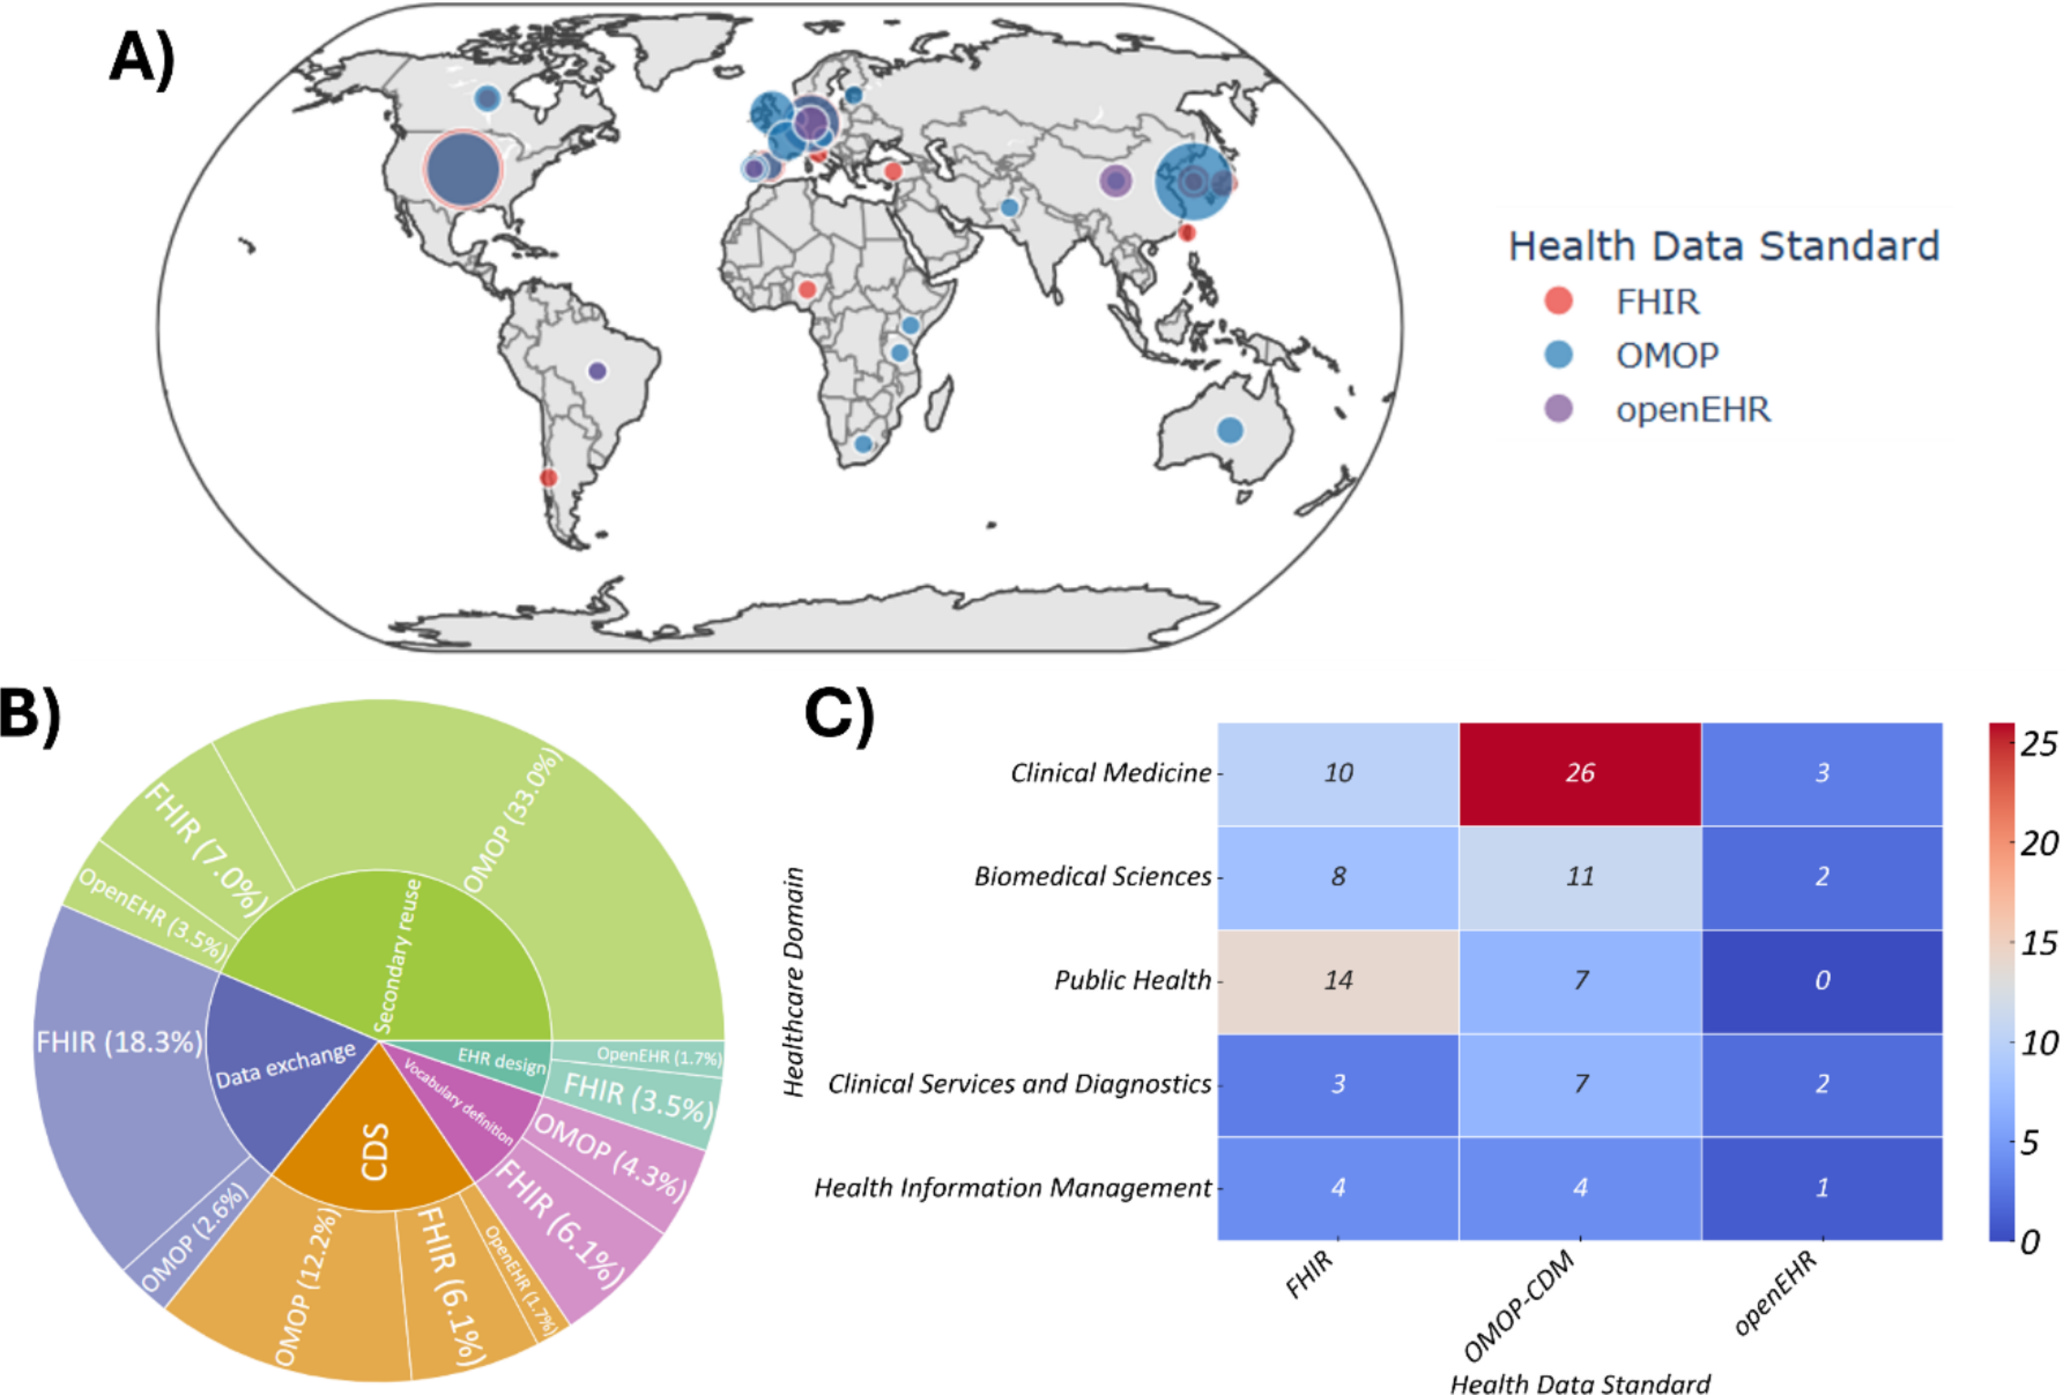
\includegraphics[width=\textwidth]{figures/paper1/fig2-overview.jpg}
\caption{Overview of the included studies A) Geographical distribution B) Distribution of the objectives, divided for each health data standard C) Healthcare domain in which health data standards are applied.}
\label{fig:paper1_overview}
\end{figure}

\subsubsection{Data extraction}
\label{sec:paper1_data_extraction}

The primary objective of this research was to outline the application of major health data standards (i.e., FHIR, OMOP-CDM, and openEHR) for real-world applications. To achieve this, we identified five key categories to clarify the context in which health data standards are used. These categories are defined as follows:

\begin{itemize}
  \item Data Exchange: The seamless transfer of health information between different systems or organizations while ensuring data accuracy, security, and interoperability.
  \item Clinical Decision Support: Enhancing clinical workflows by providing tools and recommendations to assist healthcare professionals in making informed decisions.
  \item Vocabulary Definition: Establishing terminologies and codes to ensure consistency in the representation and interpretation of clinical and administrative data.
  \item Data Reuse: Leveraging health data previously collected for patient care to pursue secondary objectives such as research, quality improvement, and public health surveillance.
  \item EHR Design: Structuring and developing electronic health records to ensure efficient data capture, usability, and interoperability.
\end{itemize}

Furthermore, we identified five major health application domains in the included studies, which were used to categorize the reviewed literature:

\begin{itemize}
  \item[i)] Clinical Medicine, including all studies about clinical and their respective applications.
  \item[ii)] Clinical Services and Diagnostics, covering studies related to healthcare delivery processes, diagnostic methodologies, and technology-supported clinical care.
  \item[iii)] Public Health, including epidemiological studies, health surveillance, and population health management.
  \item[iv)] Health Information Management, addressing data governance, interoperability frameworks, and data standardization strategies.
  \item[v)] Biomedical Sciences, focusing on bioinformatics, translational research, and the integration of health data into biomedical research.
\end{itemize}

Data extraction was led by the first author (AM), who coordinated the process and harmonized the results, with active participation from the full team in defining categories, reviewing data, and resolving ambiguities. Category selections were iteratively refined through team discussions before AM finalized the structure. Studies identified as eligible for this review have been synthesized using tables and figures to facilitate a clear understanding of the key findings. The study characteristics and outcome data will be presented in tables, resulting in aggregated information about i) General overview of the studies, ii) Dataset characteristics, iii) adopted ETL tools, and iv) Data Standard Maturity and Adoption.

\subsection{Results}
\label{sec:paper1_results}

From the systematic query of the five scientific databases, a total of 2102 records were retrieved. Before the title and abstract screening, we removed 1157 duplicate entries. Subsequently, 945 studies underwent title and abstract screening, removing a total of 716 records because they did not meet the inclusion criteria. The remaining 229 records were assessed based on their full text. Finally, 99 studies met all the inclusion criteria and were selected for further analysis. The PRISMA diagram in Fig.~\ref{fig:paper1_prisma} illustrates the complete study selection process.

Table~\ref{tab:paper1_summary} provides an overview of the included studies, specifying the study location, the standard the article is focused on, the scale at which the standardization procedure was applied, and the authors' stated objectives for applying the standard, both as described in natural language as reported in the article and as classified into the five categories defined in this review; lastly, the table includes information regarding the standard application domain, specifying if the standardization was implemented for research or clinical purposes, the health domain concerning the standardization procedure, and whether the application involved primary or secondary data use.

To enhance transparency and enable sorting and filtering of the data, the full version of Table~\ref{tab:paper1_summary} has been deposited on Zenodo. The repository \cite{marfoglia_challenges_data_2026} includes Table 1\_extended, containing the complete data extraction with detailed annotations, as well as Table 1\_summary, corresponding to the condensed version presented in the manuscript.

\subsubsection{What are the main characteristics and applications of standardized health data?}
\label{sec:paper1_results_characteristics}

The included studies were conducted across different geographical locations (Fig.~\ref{fig:paper1_overview}A), with a significant presence of high-income countries (i.e., United States, Germany, Korea, Japan). In terms of implementation scale, 31 studies \cite{li_configurable_2022,cai_advancing_2023,chechulina_semi-automated_2023,dolin_sync_2023,espinoza_development_2023,guo_development_2023,kempf_how_2023,song_implementation_2023,bae_coronary_2022,castano_identification_2022,jung_patient-level_2022,mcguinness_extraction_2021,spotnitz_patient_2022,yu_developing_2022,gomes_representation_2021,de_analyzing_2021,gruendner_framework_2021,guinez-molinos_interoperable_2021,khalifa_interoperable_2021,kim_transforming_2021,lenert_automated_2021,li_patient-screening_2021,mishra_modified_2021,oliveira_openehr_2021,paris_transformation_2021,seong_fast_2021,thayer_human-centered_2021,tian_application_2021,xiao_development_2021,zong_modeling_2021,wang_sociodemographic_2022} out of 97 (32\%) were conducted at a single-center level, 41 studies \cite{bennett2023mimic,junior_integrating_2022,raventos_transforming_2023,chukwu_standardizing_2022,bhattacharjee_inspire_2024,henke_assessing_2023,jones_real_2024,kiwuwa-muyingo_enabling_2023,kohler_eos_2023,oliver_introducing_2023,park_cancer_2023,seol_effect_2023,sinaci2023data,yu_integrating_2023,almeida_bicenter-ad_2022,bathelt_opportunities_2022,bradshaw_garde_2022,byun_analysis_2022,bialke_fhir_2022,choi_conversion_2022,lazarova_interoperable_2022,papez_transforming_2023,phuong_extracting_2021,roman-villaran_personalized_2022,sommer_structured_2022,tan_applying_2022,yoo_transforming_2022,almeida_methodology_2021,almeida_two-stage_2021,biedermann_standardizing_2021,gonzalez-castro_caside_2021,gulden_prototypical_2021,kawamoto_establishing_2021,kim_risk_2021,lamer_transforming_2021,mun_real-world_2021,nestsiarovich_predictors_2021,papez_transforming_2021,wesley_novel_2021,khalid_standardized_2021,wulff_transformation_2021} (42\%) involved more than one center, while 25 studies \cite{sadsad_computable_2023,ulgu_nationwide_2024,baumgartner_health_2024,phelan_beyond_2024,shehab_national_2024,ward_omop_2024,carus_mapping_2023,mayer_learning_2023,kim_scalable_2023,mayer_conversion_2023,oja_transforming_2023,peng_etl-process_2023,rinaldi_towards_2023,stellmach_creation_2023,bae_development_2022,carus_mapping_2022,delanerolle_methodological_2022,gruendner_architecture_2022,jung_shared_2022,rosenau_generation_2022,dolin_vcf2fhir_2021_p1,sathappan_transformation_2021,park_worker-centered_2021,seong_incorporation_2021,sun_building_2021} (26\%) were conducted on a national level. Information on the implementation scale was not reported in two of the 99 included studies. Regarding the type of health data standard adopted, more than half of the studies included (56 articles \cite{sadsad_computable_2023,cai_advancing_2023,chechulina_semi-automated_2023,guo_development_2023,kempf_how_2023,bae_coronary_2022,castano_identification_2022,jung_patient-level_2022,spotnitz_patient_2022,yu_developing_2022,kim_transforming_2021,lenert_automated_2021,paris_transformation_2021,wang_sociodemographic_2022,junior_integrating_2022,raventos_transforming_2023,bhattacharjee_inspire_2024,henke_assessing_2023,kiwuwa-muyingo_enabling_2023,kohler_eos_2023,oliver_introducing_2023,park_cancer_2023,seol_effect_2023,yu_integrating_2023,almeida_bicenter-ad_2022,bathelt_opportunities_2022,byun_analysis_2022,choi_conversion_2022,papez_transforming_2023,phuong_extracting_2021,tan_applying_2022,yoo_transforming_2022,almeida_methodology_2021,almeida_two-stage_2021,biedermann_standardizing_2021,kim_risk_2021,lamer_transforming_2021,mun_real-world_2021,nestsiarovich_predictors_2021,papez_transforming_2021,khalid_standardized_2021,baumgartner_health_2024,ward_omop_2024,carus_mapping_2023,mayer_learning_2023,kim_scalable_2023,mayer_conversion_2023,oja_transforming_2023,peng_etl-process_2023,carus_mapping_2022,delanerolle_methodological_2022,sathappan_transformation_2021,seong_incorporation_2021}, 57\%) adopted OMOP-CDM as health data standard, followed by 39 studies \cite{bennett2023mimic,ulgu_nationwide_2024,dolin_sync_2023,song_implementation_2023,mcguinness_extraction_2021,de_analyzing_2021,gruendner_framework_2021,guinez-molinos_interoperable_2021,khalifa_interoperable_2021,lenert_automated_2021,mishra_modified_2021,seong_fast_2021,thayer_human-centered_2021,xiao_development_2021,zong_modeling_2021,chukwu_standardizing_2022,jones_real_2024,sinaci2023data,bradshaw_garde_2022,bialke_fhir_2022,lazarova_interoperable_2022,roman-villaran_personalized_2022,gonzalez-castro_caside_2021,gulden_prototypical_2021,kawamoto_establishing_2021,wesley_novel_2021,phelan_beyond_2024,shehab_national_2024,peng_etl-process_2023,rinaldi_towards_2023,stellmach_creation_2023,bae_development_2022,gruendner_architecture_2022,gruendner_architecture_2022,jung_shared_2022,rosenau_generation_2022,dolin_vcf2fhir_2021_p1,park_worker-centered_2021,eisenstein_economic_2022,tang_creating_2023} (39\%) related to FHIR, and 8 studies \cite{li_configurable_2022,gomes_representation_2021,li_patient-screening_2021,oliveira_openehr_2021,tian_application_2021,kohler_eos_2023,sommer_structured_2022,wulff_transformation_2021} (8\%) focused on openEHR. The sum goes beyond the 99 included studies because some papers explored more than one standard.

The adoption of health data standards was primarily driven by data reuse, accounting for 46 studies \cite{bennett2023mimic,chechulina_semi-automated_2023,espinoza_development_2023,guo_development_2023,song_implementation_2023,yu_developing_2022,gruendner_framework_2021,kim_transforming_2021,lenert_automated_2021,li_patient-screening_2021,paris_transformation_2021,tian_application_2021,junior_integrating_2022,raventos_transforming_2023,bhattacharjee_inspire_2024,kohler_eos_2023,oliver_introducing_2023,park_cancer_2023,sinaci2023data,yu_integrating_2023,almeida_bicenter-ad_2022,bathelt_opportunities_2022,choi_conversion_2022,papez_transforming_2023,phuong_extracting_2021,tan_applying_2022,yoo_transforming_2022,almeida_methodology_2021,almeida_two-stage_2021,biedermann_standardizing_2021,gonzalez-castro_caside_2021,lamer_transforming_2021,papez_transforming_2021,wesley_novel_2021,khalid_standardized_2021,wulff_transformation_2021,baumgartner_health_2024,ward_omop_2024,carus_mapping_2023,mayer_learning_2023,mayer_conversion_2023,oja_transforming_2023,peng_etl-process_2023,delanerolle_methodological_2022,sathappan_transformation_2021,sun_building_2021} (47\%), followed by applications in clinical decision support (CDS) with 23 studies \cite{li_configurable_2022,ulgu_nationwide_2024,dolin_sync_2023,kempf_how_2023,bae_coronary_2022,castano_identification_2022,jung_patient-level_2022,mcguinness_extraction_2021,spotnitz_patient_2022,wang_sociodemographic_2022,kiwuwa-muyingo_enabling_2023,seol_effect_2023,bradshaw_garde_2022,byun_analysis_2022,roman-villaran_personalized_2022,sommer_structured_2022,tan_applying_2022,kim_risk_2021,mun_real-world_2021,nestsiarovich_predictors_2021,gruendner_architecture_2022} (23\%), data exchange with 23 studies \cite{song_implementation_2023,guinez-molinos_interoperable_2021,lenert_automated_2021,mishra_modified_2021,seong_fast_2021,xiao_development_2021,zong_modeling_2021,jones_real_2024,bialke_fhir_2022,lazarova_interoperable_2022,almeida_methodology_2021,gulden_prototypical_2021,wesley_novel_2021,phelan_beyond_2024,shehab_national_2024,kim_scalable_2023,bae_development_2022,gruendner_architecture_2022,jung_shared_2022,dolin_vcf2fhir_2021_p1,park_worker-centered_2021,eisenstein_economic_2022,tang_creating_2023} (23\%), vocabulary definition with 12 studies \cite{cai_advancing_2023,de_analyzing_2021,khalifa_interoperable_2021,chukwu_standardizing_2022,henke_assessing_2023,choi_conversion_2022,gonzalez-castro_caside_2021,rinaldi_towards_2023,stellmach_creation_2023,carus_mapping_2022,rosenau_generation_2022,seong_incorporation_2021} (12\%), and EHR design with 6 studies \cite{gomes_representation_2021,oliveira_openehr_2021,thayer_human-centered_2021,lazarova_interoperable_2022,kawamoto_establishing_2021,park_worker-centered_2021} (6\%); also in this case the sum is more than 99 studies because some papers had more than one objective. The distribution of specific health data standards varied across these categories. FHIR was the most implemented standard for data exchange, vocabulary definition, and EHR design, while OMOP-CDM was predominantly used for data reuse and CDS applications (Fig.~\ref{fig:paper1_overview}B).

Regarding the application domain, 86 studies \cite{bennett2023mimic,sadsad_computable_2023,cai_advancing_2023,chechulina_semi-automated_2023,dolin_sync_2023,espinoza_development_2023,guo_development_2023,kempf_how_2023,bae_coronary_2022,castano_identification_2022,jung_patient-level_2022,mcguinness_extraction_2021,spotnitz_patient_2022,yu_developing_2022,gomes_representation_2021,de_analyzing_2021,gruendner_framework_2021,khalifa_interoperable_2021,kim_transforming_2021,lenert_automated_2021,li_patient-screening_2021,oliveira_openehr_2021,paris_transformation_2021,seong_fast_2021,tian_application_2021,xiao_development_2021,zong_modeling_2021,wang_sociodemographic_2022,junior_integrating_2022,raventos_transforming_2023,chukwu_standardizing_2022,bhattacharjee_inspire_2024,henke_assessing_2023,jones_real_2024,kiwuwa-muyingo_enabling_2023,kohler_eos_2023,oliver_introducing_2023,park_cancer_2023,seol_effect_2023,sinaci2023data,yu_integrating_2023,almeida_bicenter-ad_2022,bathelt_opportunities_2022,byun_analysis_2022,bialke_fhir_2022,choi_conversion_2022,papez_transforming_2023,phuong_extracting_2021,roman-villaran_personalized_2022,sommer_structured_2022,tan_applying_2022,yoo_transforming_2022,almeida_methodology_2021,almeida_two-stage_2021,biedermann_standardizing_2021,gonzalez-castro_caside_2021,gulden_prototypical_2021,kim_risk_2021,lamer_transforming_2021,mun_real-world_2021,nestsiarovich_predictors_2021,papez_transforming_2021,khalid_standardized_2021,wulff_transformation_2021,baumgartner_health_2024,phelan_beyond_2024,ward_omop_2024,carus_mapping_2023,mayer_learning_2023,kim_scalable_2023,mayer_conversion_2023,oja_transforming_2023,peng_etl-process_2023,rinaldi_towards_2023,stellmach_creation_2023,carus_mapping_2022,delanerolle_methodological_2022,gruendner_architecture_2022,rosenau_generation_2022,dolin_vcf2fhir_2021_p1,sathappan_transformation_2021,park_worker-centered_2021,seong_incorporation_2021,sun_building_2021,eisenstein_economic_2022,tang_creating_2023} (87\%) were conducted in research settings, with the remaining 13 articles \cite{li_configurable_2022,ulgu_nationwide_2024,song_implementation_2023,guinez-molinos_interoperable_2021,mishra_modified_2021,thayer_human-centered_2021,bradshaw_garde_2022,lazarova_interoperable_2022,kawamoto_establishing_2021,wesley_novel_2021,shehab_national_2024,bae_development_2022,jung_shared_2022} (13\%) described applications in clinical contexts. The most frequent health domain was represented by clinical medicine, with 39 studies \cite{reinecke_usage_2021,kapitan_data_2025,page_prisma_2021,ouzzani_rayyan_2016,tsafnat_converge_2024,noauthor_repowereu_2022,dolin_sync_2023,bae_coronary_2022,mcguinness_extraction_2021,spotnitz_patient_2022,yu_developing_2022,de_analyzing_2021,gruendner_framework_2021,khalifa_interoperable_2021,kim_transforming_2021,lenert_automated_2021,seong_fast_2021,tian_application_2021,xiao_development_2021,bhattacharjee_inspire_2024,park_cancer_2023,almeida_bicenter-ad_2022,byun_analysis_2022,bialke_fhir_2022,tan_applying_2022,yoo_transforming_2022,almeida_two-stage_2021,biedermann_standardizing_2021,kawamoto_establishing_2021,kim_risk_2021,lamer_transforming_2021,mun_real-world_2021,nestsiarovich_predictors_2021,baumgartner_health_2024,shehab_national_2024,carus_mapping_2023} (39\%), followed by 20 studies \cite{li_configurable_2022,chechulina_semi-automated_2023,dolin_sync_2023,mcguinness_extraction_2021,gruendner_framework_2021,li_patient-screening_2021,mishra_modified_2021,kohler_eos_2023,bradshaw_garde_2022,lazarova_interoperable_2022,sommer_structured_2022,yoo_transforming_2022,khalid_standardized_2021,phelan_beyond_2024,ward_omop_2024,mayer_conversion_2023,rinaldi_towards_2023,park_worker-centered_2021} (20\%) about public health, 19 articles \cite{kempf_how_2023,song_implementation_2023,castano_identification_2022,lenert_automated_2021,thayer_human-centered_2021,wang_sociodemographic_2022,chukwu_standardizing_2022,kiwuwa-muyingo_enabling_2023,oliver_introducing_2023,bathelt_opportunities_2022,byun_analysis_2022,bialke_fhir_2022,phuong_extracting_2021,roman-villaran_personalized_2022,almeida_methodology_2021,almeida_two-stage_2021,lamer_transforming_2021} (19\%) in biomedical sciences, 12 studies \cite{guinez-molinos_interoperable_2021,khalifa_interoperable_2021,seong_fast_2021,seol_effect_2023,gonzalez-castro_caside_2021,nestsiarovich_predictors_2021,papez_transforming_2021,shehab_national_2024,kim_scalable_2023,rosenau_generation_2022} (12\%) in clinical services and diagnostics, and 9 studies \cite{ulgu_nationwide_2024,guo_development_2023,bae_coronary_2022,oliveira_openehr_2021,jones_real_2024,almeida_bicenter-ad_2022,gulden_prototypical_2021,dolin_vcf2fhir_2021_p1,sun_building_2021} (9\%) in Health Information Management. Also from this perspective, the distribution of health data standards varied considerably: OMOP-CDM was the most used standard for clinical medicine applications, while FHIR was the most used for Public Health applications (Fig.~\ref{fig:paper1_overview}C). Finally, 90 out of 99 studies (91\%) utilized health data standards for secondary purposes, using existing data or tools for new objectives other than the original intent (direct patient care).

Fig.~\ref{fig:paper1_dataset_magnitude} shows the size of the standardized datasets in terms of records, using the three different health data standards. It appears that OMOP-CDM works with large datasets, being the most represented standard in datasets with more than 100 records. FHIR has been used both for small and large datasets. openEHR applies in settings with moderate-sized datasets (i.e., between 100 and 1 M records).

\begin{figure}[tbp]
\centering
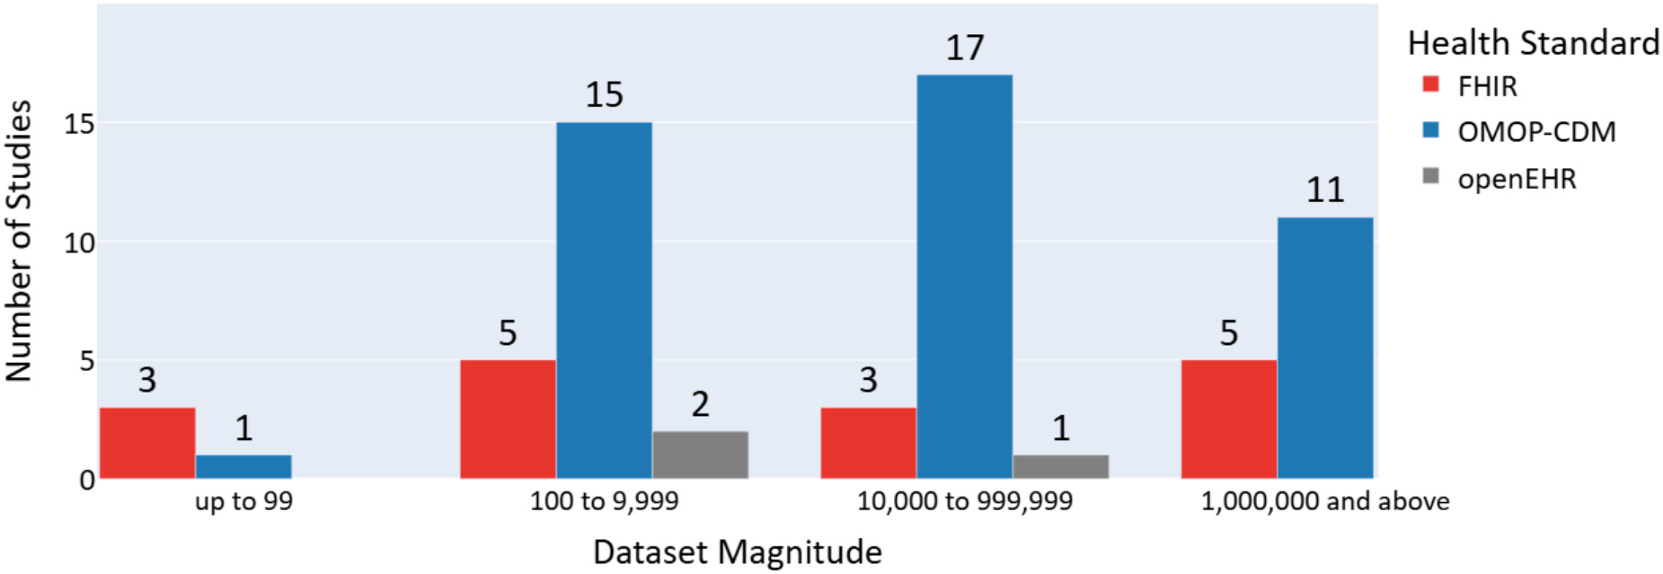
\includegraphics[width=\textwidth]{figures/paper1/fig3-dataset-magnitude.jpg}
\caption{Distribution of dataset magnitude across health data standards. Note that multiple standards might be used within the same study, meaning that counts are not mutually exclusive.}
\label{fig:paper1_dataset_magnitude}
\end{figure}

\subsubsection{How is health data standardization achieved?}
\label{sec:paper1_results_standardization}

The reviewed studies achieved health data standardization by leveraging specialized ETL tools, which aid in data cleaning, mapping, and validation. Among the 99 studies, only 15 articles \cite{bennett2023mimic,espinoza_development_2023,guo_development_2023,paris_transformation_2021,bhattacharjee_inspire_2024,almeida_bicenter-ad_2022,papez_transforming_2023,almeida_two-stage_2021,biedermann_standardizing_2021,lamer_transforming_2021,papez_transforming_2021,khalid_standardized_2021,mayer_conversion_2023,delanerolle_methodological_2022,tang_creating_2023} (15\%) provide comprehensive information about the specific ETL tools used, while 37 studies \cite{li_configurable_2022,ulgu_nationwide_2024,cai_advancing_2023,chechulina_semi-automated_2023,kempf_how_2023,yu_developing_2022,de_analyzing_2021,gruendner_framework_2021,lenert_automated_2021,li_patient-screening_2021,mishra_modified_2021,tian_application_2021,xiao_development_2021,junior_integrating_2022,raventos_transforming_2023,henke_assessing_2023,kiwuwa-muyingo_enabling_2023,kohler_eos_2023,park_cancer_2023,sinaci2023data,yu_integrating_2023,bathelt_opportunities_2022,bradshaw_garde_2022,byun_analysis_2022,bialke_fhir_2022,choi_conversion_2022,phuong_extracting_2021,tan_applying_2022,almeida_methodology_2021,baumgartner_health_2024,phelan_beyond_2024,ward_omop_2024,carus_mapping_2023,oja_transforming_2023,sathappan_transformation_2021} (37\%) provide partial information, with some tools not explicitly identified.

Studies adopting OMOP-CDM leveraged commonly used tools \cite{bhattacharjee_inspire_2024,papez_transforming_2023,almeida_methodology_2021,lamer_transforming_2021,papez_transforming_2021,khalid_standardized_2021,delanerolle_methodological_2022,rosenau_generation_2022} such as White Rabbit,USAGI, Rabbit-in-a-Hat, and ACHILLES, all developed within the OHDSI ecosystem and routinely used in OMOP-CDM implementations.

In contrast, FHIR-based conversion pipelines appear to be more diverse, involving a mix of proprietary tools (e.g., SmileCDR) \cite{ulgu_nationwide_2024,lenert_automated_2021,mishra_modified_2021,sinaci2023data,bialke_fhir_2022} and open-source solutions (e.g.,HAPI FHIR) \cite{marfoglia_towards_2025,bennett2023mimic,phelan_beyond_2024}. Lastly, openEHR implementations rely on more specialized tools, such as Clinical Knowledge Manager and openEHR EL \cite{li_configurable_2022,li_patient-screening_2021,kohler_eos_2023}.

\begin{figure}[tbp]
\centering
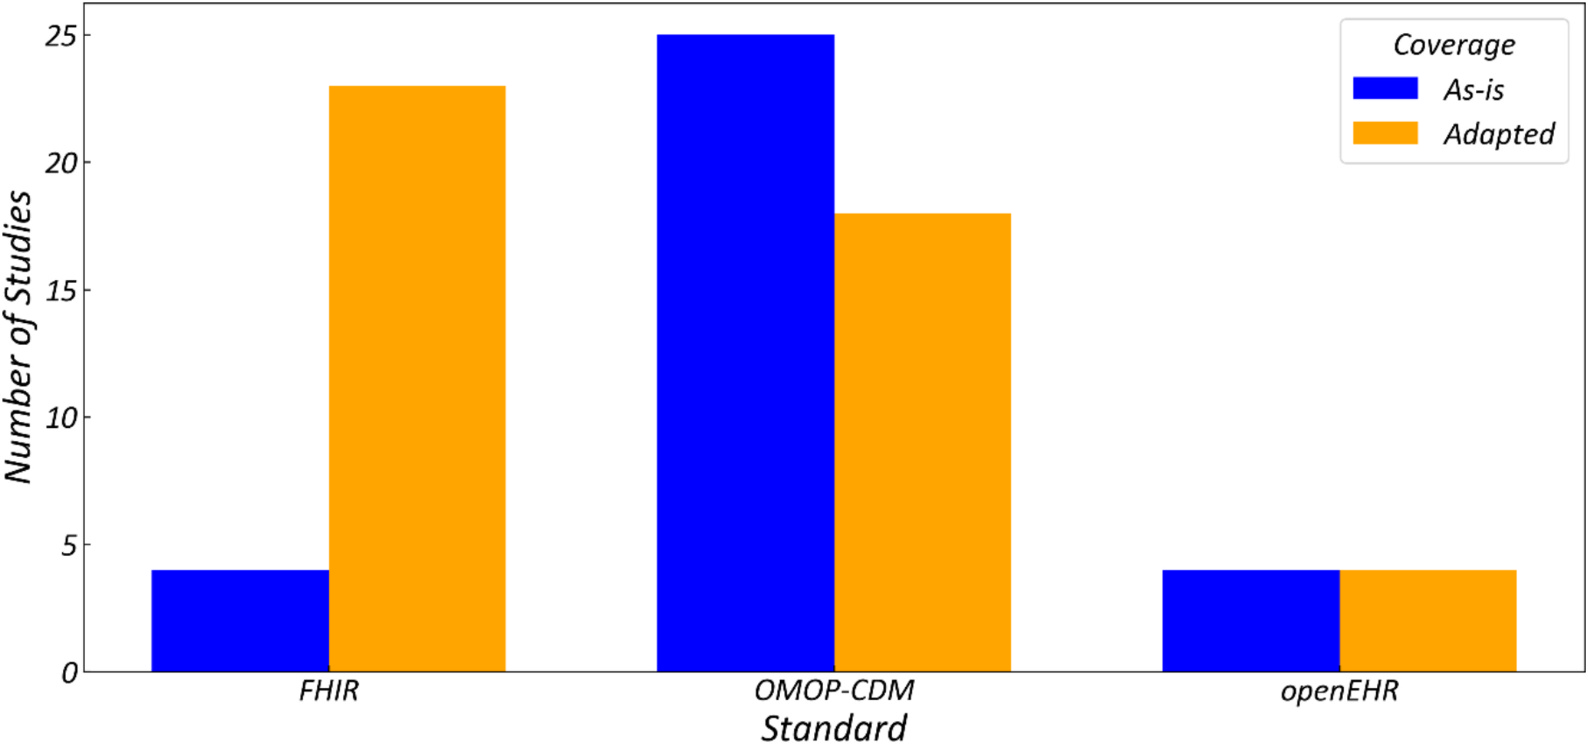
\includegraphics[width=\textwidth]{figures/paper1/fig4-coverage.jpg}
\caption{Coverage of health data standards: number of studies that used the standard as-is or adapted it.}
\label{fig:paper1_coverage}
\end{figure}

\subsubsection{How extensive is the use of standardized data in relation to the total data utilized for application implementation?}
\label{sec:paper1_results_extent}

Among the 99 studies, only 27 articles \cite{cai_advancing_2023,kempf_how_2023,jung_patient-level_2022,yu_developing_2022,kim_transforming_2021,li_patient-screening_2021,paris_transformation_2021,tian_application_2021,zong_modeling_2021,junior_integrating_2022,raventos_transforming_2023,bhattacharjee_inspire_2024,henke_assessing_2023,oliver_introducing_2023,roman-villaran_personalized_2022,almeida_methodology_2021,almeida_two-stage_2021,gulden_prototypical_2021,lamer_transforming_2021,mayer_learning_2023,kim_scalable_2023,mayer_conversion_2023,carus_mapping_2022,rosenau_generation_2022,sathappan_transformation_2021} (27\%) provided information related to the coverage of the standard (i.e., the number of variables from the original dataset mapped in the selected standard), while 77 studies \cite{bennett2023mimic,li_configurable_2022,cai_advancing_2023,chechulina_semi-automated_2023,dolin_sync_2023,espinoza_development_2023,guo_development_2023,kempf_how_2023,song_implementation_2023,bae_coronary_2022,castano_identification_2022,jung_patient-level_2022,mcguinness_extraction_2021,spotnitz_patient_2022,gomes_representation_2021,khalifa_interoperable_2021,kim_transforming_2021,li_patient-screening_2021,oliveira_openehr_2021,paris_transformation_2021,seong_fast_2021,thayer_human-centered_2021,tian_application_2021,xiao_development_2021,zong_modeling_2021,junior_integrating_2022,raventos_transforming_2023,chukwu_standardizing_2022,bhattacharjee_inspire_2024,henke_assessing_2023,kohler_eos_2023,oliver_introducing_2023,seol_effect_2023,sinaci2023data,yu_integrating_2023,bathelt_opportunities_2022,bialke_fhir_2022,choi_conversion_2022,papez_transforming_2023,phuong_extracting_2021,roman-villaran_personalized_2022,sommer_structured_2022,tan_applying_2022,almeida_methodology_2021,almeida_two-stage_2021,biedermann_standardizing_2021,gonzalez-castro_caside_2021,gulden_prototypical_2021,kawamoto_establishing_2021,kim_risk_2021,lamer_transforming_2021,mun_real-world_2021,nestsiarovich_predictors_2021,papez_transforming_2021,wesley_novel_2021,khalid_standardized_2021,wulff_transformation_2021,phelan_beyond_2024,shehab_national_2024,ward_omop_2024,carus_mapping_2023,mayer_learning_2023,kim_scalable_2023,mayer_conversion_2023,oja_transforming_2023,rinaldi_towards_2023,stellmach_creation_2023,bae_development_2022,delanerolle_methodological_2022,gruendner_architecture_2022,jung_shared_2022,rosenau_generation_2022,dolin_vcf2fhir_2021_p1,sathappan_transformation_2021,seong_incorporation_2021,sun_building_2021,tang_creating_2023} (78\%) clearly stated whether the standard was used in its original form (i.e., as-is) or if it was extended (i.e., adapted). Indeed, Fig.~\ref{fig:paper1_coverage} reports that, among these 77 studies, 27 \cite{bennett2023mimic,dolin_sync_2023,song_implementation_2023,mcguinness_extraction_2021,khalifa_interoperable_2021,seong_fast_2021,thayer_human-centered_2021,xiao_development_2021,zong_modeling_2021,chukwu_standardizing_2022,sinaci2023data,bialke_fhir_2022,roman-villaran_personalized_2022,gulden_prototypical_2021,kawamoto_establishing_2021,wesley_novel_2021,phelan_beyond_2024,shehab_national_2024,rinaldi_towards_2023,stellmach_creation_2023,bae_development_2022,gruendner_architecture_2022,jung_shared_2022,rosenau_generation_2022,dolin_vcf2fhir_2021_p1} (35\%) use FHIR, 44 \cite{cai_advancing_2023,chechulina_semi-automated_2023,guo_development_2023,kempf_how_2023,bae_coronary_2022,castano_identification_2022,jung_patient-level_2022,spotnitz_patient_2022,kim_transforming_2021,paris_transformation_2021,junior_integrating_2022,raventos_transforming_2023,bhattacharjee_inspire_2024,henke_assessing_2023,kohler_eos_2023,oliver_introducing_2023,seol_effect_2023,yu_integrating_2023,bathelt_opportunities_2022,choi_conversion_2022,papez_transforming_2023,phuong_extracting_2021,tan_applying_2022,almeida_methodology_2021,almeida_two-stage_2021,biedermann_standardizing_2021,kim_risk_2021,mun_real-world_2021,nestsiarovich_predictors_2021,papez_transforming_2021,khalid_standardized_2021,ward_omop_2024,carus_mapping_2023,mayer_learning_2023,kim_scalable_2023,mayer_conversion_2023,oja_transforming_2023,stellmach_creation_2023,delanerolle_methodological_2022,sathappan_transformation_2021,seong_incorporation_2021} (57\%) use OMOP-CDM, and 8 \cite{li_configurable_2022,gomes_representation_2021,li_patient-screening_2021,oliveira_openehr_2021,tian_application_2021,kohler_eos_2023,sommer_structured_2022,wulff_transformation_2021} (10\%) use openEHR, resulting in more than 77 studies because two papers simultaneously used two standards. Of the 27 studies involving FHIR, 23 articles \cite{bennett2023mimic,dolin_sync_2023,song_implementation_2023,khalifa_interoperable_2021,seong_fast_2021,thayer_human-centered_2021,xiao_development_2021,zong_modeling_2021,chukwu_standardizing_2022,sinaci2023data,bialke_fhir_2022,gonzalez-castro_caside_2021,gulden_prototypical_2021,kawamoto_establishing_2021,wesley_novel_2021,phelan_beyond_2024,shehab_national_2024,stellmach_creation_2023,bae_development_2022,gruendner_architecture_2022,jung_shared_2022,rosenau_generation_2022,dolin_vcf2fhir_2021_p1} (85\%) reported adapting the standard to specific use cases, often to accommodate local requirements or specialized clinical workflows. In contrast, 25 studies \cite{espinoza_development_2023,guo_development_2023,castano_identification_2022,jung_patient-level_2022,spotnitz_patient_2022,junior_integrating_2022,henke_assessing_2023,kohler_eos_2023,oliver_introducing_2023,seol_effect_2023,yu_integrating_2023,bathelt_opportunities_2022,phuong_extracting_2021,tan_applying_2022,kim_risk_2021,mun_real-world_2021,nestsiarovich_predictors_2021,khalid_standardized_2021,carus_mapping_2023,mayer_learning_2023,mayer_conversion_2023,delanerolle_methodological_2022,seong_incorporation_2021} utilizing OMOP-CDM (57\%) implemented the standard without modification, while openEHR was applied equally in both adapted \cite{gomes_representation_2021,oliveira_openehr_2021,tian_application_2021,wulff_transformation_2021} and unmodified forms \cite{li_configurable_2022,li_patient-screening_2021,kohler_eos_2023,sommer_structured_2022} (50\% each).

\subsubsection{What are the main limitations and barriers to the application of health data standards?}
\label{sec:paper1_results_limitations}

This subsection examines the key limitations of each healthcare standard based on insights gathered from the reviewed papers. Rather than addressing general challenges, we focused on issues arising from unique standards.

One of the critical barriers to OMOP-CDM adoption is its inherent complexity. The OMOP-CDM standard can be overwhelming, especially when harmonizing cohorts across different institutions.

OMOP-CDM complexity primarily stems from its data model architecture and transformation requirements. Originally designed for large-scale harmonization of heterogeneous, longitudinal EHR and administrative datasets, OMOP-CDM features an extensive relational schema with more than forty interrelated tables. The transformation of primary-care data into the OMOP structure has been shown to require complex structural mapping and extensive vocabulary alignment due to the heterogeneity of local and country-specific data sources \cite{fruchart_transforming_2024}. Evidence from comparative mapping studies indicates that the ETL phase remains the most resource-intensive aspect of OMOP adoption, demanding reconciliation of diverse terminologies and encounter representations \cite{peng_etl-process_2023,papez_transforming_2023}. Similar findings were reported for multi-country primary-care data transformations, where differences in coding systems and record granularity significantly increased implementation effort \cite{kent_common_2021}.

In contrast, FHIR employs a modular, resource-oriented architecture optimized for real-time data exchange rather than retrospective analytics, resulting in a lighter implementation burden at the interface level. openEHR, by comparison, provides a semantic modeling framework based on archetypes that ensures internal consistency but is less focused on large-scale ETL and analytic workflows.

Additionally, the OMOP-CDM structure lacks crucial clinical details, such as cognitive scores and genetic markers \cite{byun_analysis_2022}. Its patient-centric design also challenges mapping administrative and institutional data, making it less suitable for use cases requiring detailed operational insights. Another limitation is the absence of real-time data ingestion and patient re-identification mechanisms \cite{paris_transformation_2021}, restricting OMOP-CDM applicability in time-sensitive studies. Furthermore, while the OHDSI ecosystem provides robust analytical tools like ATHENA \cite{seong_incorporation_2021}, these tools demand significant computational resources, posing a barrier for institutions with limited infrastructure.

Regarding FHIR, its flexibility can be a double-edged sword \cite{xiao_development_2021,sinaci2023data,kramer_reducing_2022}. While its adaptable structure allows for personalization across different domains, this feature can lead to inconsistencies between implementations. The extension mechanism, though essential for customization, often complicates interoperability on a global scale. Another limitation is data fragmentation \cite{gonzalez-castro_caside_2021}: information is often scattered across multiple FHIR resources and extensions \cite{xiao_development_2021},making it difficult to perform efficient searches, especially without advanced server capabilities \cite{bennett2023mimic}. This latter negative aspect is also due to the lack of native support for complex multi-criteria searches \cite{gruendner_framework_2021}. Without a dedicated preprocessing module integrated into the FHIR server \cite{song_implementation_2023}, the execution of advanced queries remains cumbersome \cite{gruendner_architecture_2022}, particularly in high-volume data environments \cite{gruendner_framework_2021}. Finally, the standard follows the 80/20 rule \cite{stellmach_creation_2023} --- designed to cover 80\% of use cases while leaving the remaining 20\% to custom extensions --- which means it may not capture the full granularity of clinical data, potentially leading to data loss.

None of the authors in the studies adopting openEHR reported any limitations; therefore, no limitations have been included in this review for those studies.

\subsection{Discussion}
\label{sec:paper1_discussion}

In recent years, the adoption of health data standards has become increasingly important for achieving interoperability, facilitating clinical research, and supporting innovation in healthcare. This systematic review aimed to examine the maturity of health data standard adoption in real-world contexts, focusing on three major standards: FHIR, OMOP-CDM, and openEHR. Through the analysis of 99 selected studies, we explored the specific characteristics, applications, and limitations of these standards, as well as the broader challenges associated with their implementation. Our findings may offer a broad overview of how these standards contribute to healthcare delivery and research, highlighting both their complementary strengths and persistent barriers to widespread adoption.

Indeed, the different health data standards are not competing but complementary building blocks of a modern, interoperable health data ecosystem. Each standard plays a distinct and valuable role: openEHR to persist data, FHIR to transfer data between organizations, and OMOP-CDM to find insights into the data \cite{tsafnat_converge_2024}. The synergistic integration of these standards has shown tangible benefits across the full clinical data lifecycle. For example, Kohler et al. \cite{kohler_eos_2023} proposed a framework that integrates openEHR with OMOP-CDM. Their approach used openEHR for semantic precision and representational consistency at the care-site level and subsequently transformed openEHR archetypes into OMOP-CDM-conformant datasets, enabling standardized data reuse for research. Similarly, Peng et al. \cite{peng_etl-process_2023} developed an ETL process for harmonizing FHIR-based hospital data with OMOP-CDM. In their implementation, FHIR supported national interoperability requirements within the German Medical Informatics Initiative, while OMOP-CDM facilitated participation in international research networks such as OHDSI and DARWIN EU. Furthermore, Lenert et al. \cite{lenert_automated_2021} developed an automated approach to enable near real-time, multi-institutional data sharing for COVID-19 research. FHIR served as a canonical, real-time data exchange model compliant with U.S. interoperability regulations, while OMOP-CDM provided a harmonized analytical format suitable for research networks, including the National COVID Cohort Collaborative (N3C).

Moreover, this work underscores the critical importance of data standards in catalyzing innovation across various domains within healthcare. Among these, FHIR has emerged as a key enabler of public health applications, being featured in 14 \cite{bennett2023mimic,song_implementation_2023,de_analyzing_2021,mishra_modified_2021,xiao_development_2021,jones_real_2024,sinaci2023data,kawamoto_establishing_2021,wesley_novel_2021,phelan_beyond_2024,shehab_national_2024,peng_etl-process_2023,gruendner_architecture_2022,park_worker-centered_2021} of the 39 relevant studies (36\%). Similarly, the OMOP-CDM robust relational data model was highlighted in 26 \cite{sadsad_computable_2023,chechulina_semi-automated_2023,guo_development_2023,kempf_how_2023,bae_coronary_2022,castano_identification_2022,jung_patient-level_2022,spotnitz_patient_2022,kim_transforming_2021,wang_sociodemographic_2022,park_cancer_2023,seol_effect_2023,yu_integrating_2023,byun_analysis_2022,choi_conversion_2022,tan_applying_2022,yoo_transforming_2022,almeida_two-stage_2021,biedermann_standardizing_2021,nestsiarovich_predictors_2021,papez_transforming_2021,baumgartner_health_2024,carus_mapping_2023,carus_mapping_2022} of 55 studies (47\%) for its capacity to support complex, longitudinal analyses, reinforcing its utility in clinical research. Across the three standards examined, Clinical Medicine surfaced as the most prominent application domain, appearing in 39 \cite{sadsad_computable_2023,li_configurable_2022,ulgu_nationwide_2024,chechulina_semi-automated_2023,espinoza_development_2023,guo_development_2023,kempf_how_2023,bae_coronary_2022,castano_identification_2022,jung_patient-level_2022,mcguinness_extraction_2021,spotnitz_patient_2022,kim_transforming_2021,lenert_automated_2021,thayer_human-centered_2021,zong_modeling_2021,wang_sociodemographic_2022,chukwu_standardizing_2022,park_cancer_2023,seol_effect_2023,yu_integrating_2023,bradshaw_garde_2022,byun_analysis_2022,choi_conversion_2022,lazarova_interoperable_2022,roman-villaran_personalized_2022,sommer_structured_2022,tan_applying_2022,yoo_transforming_2022,almeida_two-stage_2021,biedermann_standardizing_2021,gonzalez-castro_caside_2021,nestsiarovich_predictors_2021,papez_transforming_2021,baumgartner_health_2024,carus_mapping_2023,rinaldi_towards_2023,carus_mapping_2022,almeida_bicenter-ad_2022} of 99 studies (39\%). This dominance likely reflects the inherently structured and protocol-driven nature of clinical workflows, which naturally lend themselves to data harmonization efforts.

FHIR modular architecture, centered on reusable resources, supports flexible system design and incremental updates \cite{park_worker-centered_2021}, enabling scalable and maintainable implementations across clinical care \cite{guinez-molinos_interoperable_2021,gulden_prototypical_2021}, public health, and research. Its strength lies in standardizing profiles and terminologies \cite{bennett2023mimic,rinaldi_towards_2023}, facilitating real-time access to complex data, including patient-reported outcomes \cite{wesley_novel_2021} and genomic information \cite{dolin_sync_2023,khalifa_interoperable_2021,seong_fast_2021,stellmach_creation_2023,dolin_vcf2fhir_2021_p1}, vital for modern clinical decision-making. FHIR is particularly well-suited to low- and middle-income countries \cite{chukwu_standardizing_2022}, where affordability and flexibility are essential. Growing adoption by major EHR vendors \cite{thayer_human-centered_2021} has further simplified its integration into existing health systems, especially in regions like Europe and the U.S. \cite{xiao_development_2021,jones_real_2024}, where supportive regulatory frameworks, including centralized IRBs \cite{eisenstein_economic_2022}, are accelerating its uptake.

OMOP-CDM stands out for its excellence in clinical decision support and secondary use of health data. Its relational model supports complex, longitudinal analyses across large datasets \cite{bhattacharjee_inspire_2024,ward_omop_2024}, making it especially valuable for clinical research and predictive and machine learning applications \cite{guo_development_2023,kim_transforming_2021,bathelt_opportunities_2022,nestsiarovich_predictors_2021}. With a mature ETL ecosystem \cite{almeida_bicenter-ad_2022} and an expanding set of analytics tools \cite{raventos_transforming_2023}, OMOP-CDM is well-suited for multi-institutional data standardization workflows where real-world data (RWD) are transformed into real-world evidence (RWE) through collaborative \cite{tan_applying_2022,mun_real-world_2021,almeida_bicenter-ad_2022} and federated analyses \cite{yu_integrating_2023,carus_mapping_2023}. Moreover, its integration with ontologies like the Human Phenotype Ontology (HPO) \cite{castano_identification_2022} extends its utility to domains such phenomics \cite{castano_identification_2022,papez_transforming_2023,khalid_standardized_2021} and oncology \cite{kempf_how_2023,park_cancer_2023,seol_effect_2023,yoo_transforming_2022,carus_mapping_2022}.

openEHR provides a robust, patient-centered standard for long-term EHR data persistence and semantic interoperability. Its two-level modeling approach \cite{wulff_transformation_2021} separates a stable reference information model from adaptable, domain-specific clinical models, thus enabling seamless collaboration between IT professionals and clinicians \cite{li_configurable_2022} within their respective domains. This separation reduces communication overhead and fosters clinically meaningful implementations \cite{wulff_transformation_2021}. Optimized for rich, longitudinal health records across a patient's lifetime, openEHR includes features such as record versioning, auditing, and the Archetype Query Language (AQL) \cite{oliveira_openehr_2021}. When combined with the Expression Language (EL) \cite{li_patient-screening_2021}, these tools enable efficient, expressive querying that can outperform traditional SQL-based methods for data retrieval and screening tasks. However, its adoption in academic literature remains limited: only 2 \cite{gomes_representation_2021,oliveira_openehr_2021} out of 8 studies (25\%) referenced its use in EHR design.

Despite the significant potential of these health data standards, several limitations persist, particularly in their ETL workflow implementation. A key observation from the reviewed studies is the inconsistent reporting of ETL tools. This lack of detail limits reproducibility and highlights a gap in the standardization of implementation processes. One of the most technically and conceptually demanding components of ETL is data mapping. This process extends well beyond structural alignment and requires interpretive judgment, contextual understanding, and domain-specific expertise. Determining whether a source variable fully corresponds to a target concept might often lead to ambiguity, particularly when integrating data collected across heterogeneous clinical settings. Mapping decisions can vary between experts, driven by differences in disciplinary background, assumptions, and local priorities, hence making data mapping an inherently subjective and resource-intensive process.

These challenges are particularly pronounced in standards such as FHIR, whose flexible and abstract resource definitions allow for multiple valid representations of the same real-world concept. While this flexibility supports extensibility and innovation, it complicates standardization and validation. The lack of external reference mappings or ``gold standards'' further exacerbates this issue. Establishing authoritative mappings would require sustained verification efforts by standard developers or regulatory bodies, which are rarely feasible in practice. Consequently, practical tools, guidelines, and consensus-driven processes within the relevant reference community become essential.

FHIR-based ETL workflows remain heterogeneous as well. Reviewed studies employed a mix of proprietary tools (e.g., SmileCDR, onFHIR.io) \cite{ulgu_nationwide_2024,lenert_automated_2021,mishra_modified_2021,sinaci2023data,bialke_fhir_2022} and open-source libraries (e.g., HAPI FHIR, SMART on FHIR) \cite{marfoglia_towards_2025,bennett2023mimic,phelan_beyond_2024}, as well as Matchbox with FHIR Mapping Language for automated data transformation using Structure Maps17,23. These tools support advanced operations such as conditional updates and adapt well to evolving data requirements. Beyond the tools gathered in this systematic literature review, the broader FHIR ecosystem includes the FHIR Tools Registry for guide publication, the Firely.NET SDK \cite{noauthor_firely_net_sdk} for.NET integration, and platforms like Simplifier.net for collaboration \cite{firely_simplifier}. Moreover, industry-grade FHIR server implementations from private companies, such as IBM (IBM\textregistered{} FHIR\textregistered{} Server) and Microsoft (FHIR Server for Azure), support the deployment of scalable solutions and provide additional capabilities, such as legacy HL7 message conversion to FHIR.

In contrast, OMOP-CDM, through the efforts of the OHDSI community in delivering such tools, demonstrates a relatively mature and cohesive ETL ecosystem \cite{bhattacharjee_inspire_2024,rosenau_generation_2022}: White Rabbit performs profiling of source datasets, summarizing structures \cite{bhattacharjee_inspire_2024,papez_transforming_2023,almeida_methodology_2021,lamer_transforming_2021,papez_transforming_2021,khalid_standardized_2021,delanerolle_methodological_2022,rosenau_generation_2022}; the Rabbit-in-a-Hat application provides a GUI for designing ETL pipelines and documenting data mapping \cite{junior_integrating_2022,raventos_transforming_2023,bhattacharjee_inspire_2024,kiwuwa-muyingo_enabling_2023,papez_transforming_2023,tan_applying_2022,lamer_transforming_2021,papez_transforming_2021,khalid_standardized_2021,delanerolle_methodological_2022}; USAGI supports the semi-automated mapping of local terminologies to OMOP-CDM standardized vocabularies \cite{cai_advancing_2023,chechulina_semi-automated_2023,guo_development_2023,raventos_transforming_2023,bhattacharjee_inspire_2024,henke_assessing_2023,kiwuwa-muyingo_enabling_2023,papez_transforming_2023,almeida_methodology_2021,almeida_two-stage_2021,lamer_transforming_2021,papez_transforming_2021,khalid_standardized_2021,ward_omop_2024,carus_mapping_2023,oja_transforming_2023,delanerolle_methodological_2022,rosenau_generation_2022,sathappan_transformation_2021,sun_building_2021}; finally, tools such as the Data Quality Dashboard (DQD) and ACHILLES allow for systematic quality checks identifying anomalies and ensuring OMOP-CDM compliance \cite{kim_transforming_2021,paris_transformation_2021,bhattacharjee_inspire_2024,papez_transforming_2023,almeida_methodology_2021,biedermann_standardizing_2021,lamer_transforming_2021,papez_transforming_2021,khalid_standardized_2021,oja_transforming_2023}.

Similarly, ETL processes involving openEHR are constrained by the technical complexity of its dual-model architecture and the limited availability of standardized tooling \cite{wulff_transformation_2021}. Only 8 studies in our review addressed openEHR ETL processes, with Clinical Knowledge Manager \cite{li_configurable_2022,kohler_eos_2023} and the openEHR Expression Language \cite{li_patient-screening_2021} being the only tools explicitly cited. Nonetheless, the ecosystem includes foundational development tools such as the ADL Workbench \cite{tian_application_2021}, Archetype Editor, EHR Server, and the opener-rm-core Java library for Reference Model integration \cite{chen_openehr_2007}.

Our findings highlight the differing natures of the selected standards. Studies using FHIR often adapt the standard --- typically by modifying existing implementation guides --- to address local or specialty-specific needs \cite{bennett2023mimic,dolin_sync_2023,song_implementation_2023,khalifa_interoperable_2021,seong_fast_2021,thayer_human-centered_2021,xiao_development_2021,zong_modeling_2021,chukwu_standardizing_2022,sinaci2023data,bialke_fhir_2022,gonzalez-castro_caside_2021,gulden_prototypical_2021,kawamoto_establishing_2021,wesley_novel_2021,phelan_beyond_2024,shehab_national_2024,stellmach_creation_2023,bae_development_2022,gruendner_architecture_2022,jung_shared_2022,rosenau_generation_2022,dolin_vcf2fhir_2021_p1}, reflecting FHIR inherent flexibility. In contrast, the rigid table structure of OMOP-CDM discourages modification; however, 33\% of the reviewed OMOP-CDM studies \cite{cai_advancing_2023,chechulina_semi-automated_2023,kempf_how_2023,kim_transforming_2021,paris_transformation_2021,raventos_transforming_2023,bhattacharjee_inspire_2024,choi_conversion_2022,papez_transforming_2023,almeida_two-stage_2021,biedermann_standardizing_2021,lamer_transforming_2021,papez_transforming_2021,ward_omop_2024,kim_scalable_2023,oja_transforming_2023} extended the model to suit medical domains or national health initiatives. openEHR, which promotes structural reuse through archetypes, was implemented without modification in about half of the analyzed studies \cite{li_configurable_2022,li_patient-screening_2021,kohler_eos_2023,sommer_structured_2022}. Due to the limited extensibility of OMOP-CDM, in some cases the concept coverage is reported to be rather low \cite{jung_patient-level_2022,yu_developing_2022}. It is noteworthy, however, that the mapped percentage is rarely reported in the articles using FHIR and openEHR standards, so it is not possible to make a comparison of variable coverage between the standards. The difference in the coverage reporting could be due to the different aims and ``cultures'' of the standard communities. FHIR is being used largely by developers for the design of efficient data exchange and clinical decision support system apps, more directed to current and future clinical data. On the other hand, OMOP-CDM users leverage massive existing datasets to be merged in a harmonized, unique clinical study, which may explain why OMOP-CDM users are more attentive to the standardization coverage.

Despite their technical maturity and complementary roles, FHIR, OMOP-CDM, and openEHR each face distinct limitations that hinder widespread adoption in healthcare settings. A key challenge is fragmentation in implementation practices. FHIR aims to enable interoperability through standardized APIs and profiles, yet inconsistent implementation across institutions, organizational disparities, and rigid mappings often result in semantic mismatches in practice \cite{xiao_development_2021,sinaci2023data,gonzalez-castro_caside_2021,kramer_reducing_2022}. While FHIR granular structure is advantageous for selective data sharing and AI applications, its layered and complex architecture poses barriers to AI integration, necessitating significant data preprocessing and transformation \cite{williams2023standardized}. OMOP-CDM, by contrast, excels in supporting large-scale research through harmonized data models and standardized vocabularies. However, the ETL process required to convert heterogeneous clinical data into OMOP-CDM is resource-intensive and technically demanding \cite{williams2023standardized,almeida_methodology_2021}, posing challenges for smaller organizations. Additionally, data transformation may lead to loss of clinical detail --- especially in domains like rare diseases --- due to the model reliance on administrative coding systems and its research-oriented design \cite{bae_coronary_2022,kohler_eos_2023,seol_effect_2023,byun_analysis_2022,papez_transforming_2023,lamer_transforming_2021,mun_real-world_2021,papez_transforming_2021,carus_mapping_2023,mayer_conversion_2023,oja_transforming_2023}. openEHR presents a different set of challenges, primarily structural rather than technical. Its archetype-based approach offers strong semantic precision and reusability, yet adoption remains limited due to its complexity and divergence from prevailing industry practices \cite{delussu_survey_2024}. The steep learning curve, the need for specialized training, and the limited alignment with cloud-native and commercial development workflows could explain its slow uptake \cite{delussu_survey_2024}. Furthermore, a lack of vendor incentives and an immature ecosystem of mapping tools between openEHR and other standards hinder broader integration \cite{delussu_survey_2024}. Performance concerns have also been noted in some studies, with openEHR systems sometimes exhibiting lower throughput compared to proprietary alternatives \cite{kryszyn_performance_2022}.

While in this paper the term maturity is used to qualitatively evaluate the degree of practical adoption and consolidation of standards in operational environments, future work may build on these findings to develop measurable criteria for maturity assessment and cross-standard comparison. Although a wide range of quantitative tools to asses technology adoption maturity exists \cite{noauthor_paho_maturity_2022,measure_evaluation_his_toolkit,noauthor_himss_maturity,liaw_digital_2021}, the content of the included papers did not allow for their comprehensive application. Moreover, as this review focused exclusively on peer-reviewed literature, our analysis did not capture evidence from non-academic sources or market-driven implementations that often represent advanced or commercially mature deployments. This introduces an inherent bias toward research-documented initiatives and may underestimate the true level of real-world standard adoption and integration, particularly in vendor-led or proprietary contexts.

Future studies on health data standard adoption could directly operationalize the frameworks to perform formal maturity assessments and comparative evaluations across standards or implementation contexts.

This systematic review has several limitations that may affect the generalizability and comprehensiveness of its findings. First, the scope was restricted to studies published within the past four years. This decision was made to prioritize recent developments, particularly those emerging in the wake of the COVID-19 pandemic, which significantly accelerated innovation in health data infrastructure. However, this temporal restriction may have led to the exclusion of earlier yet potentially influential studies. Nonetheless, the inclusion of 99 studies suggests a substantial and growing body of contemporary research in this area. Furthermore, the review may be affected by publication bias. A substantial proportion of health data standardization work occurs within private or vendor-driven settings where implementation details are rarely disclosed due to commercial or intellectual property constraints. As this study systematically analyzed peer-reviewed scientific literature, clinically deployed and commercially maintained systems were largely outside its scope. Consequently, the findings reflect research-oriented and publicly documented implementations. This limitation likely contributes to two observed patterns: (1) the predominance of research-oriented studies (87\%) \cite{bennett2023mimic,sadsad_computable_2023,cai_advancing_2023,chechulina_semi-automated_2023,dolin_sync_2023,dolin_sync_2023,espinoza_development_2023,guo_development_2023,kempf_how_2023,bae_coronary_2022,castano_identification_2022,jung_patient-level_2022,mcguinness_extraction_2021,spotnitz_patient_2022,yu_developing_2022,gomes_representation_2021,de_analyzing_2021,khalifa_interoperable_2021,kim_transforming_2021,lenert_automated_2021,oliveira_openehr_2021,paris_transformation_2021,seong_fast_2021,tian_application_2021,xiao_development_2021,zong_modeling_2021,wang_sociodemographic_2022,junior_integrating_2022,raventos_transforming_2023,chukwu_standardizing_2022,bhattacharjee_inspire_2024,henke_assessing_2023,jones_real_2024,kiwuwa-muyingo_enabling_2023,kohler_eos_2023,oliver_introducing_2023,park_cancer_2023,seol_effect_2023,sinaci2023data,yu_integrating_2023,bathelt_opportunities_2022,byun_analysis_2022,bialke_fhir_2022,choi_conversion_2022,phuong_extracting_2021,roman-villaran_personalized_2022,sommer_structured_2022,tan_applying_2022,yoo_transforming_2022,almeida_methodology_2021,almeida_two-stage_2021,biedermann_standardizing_2021,gonzalez-castro_caside_2021,gulden_prototypical_2021,kim_risk_2021,lamer_transforming_2021,lamer_transforming_2021,mun_real-world_2021,nestsiarovich_predictors_2021,papez_transforming_2021,papez_transforming_2021,khalid_standardized_2021,wulff_transformation_2021,baumgartner_health_2024,phelan_beyond_2024,ward_omop_2024,carus_mapping_2023,mayer_learning_2023,kim_scalable_2023,mayer_conversion_2023,oja_transforming_2023,peng_etl-process_2023,rinaldi_towards_2023,rinaldi_towards_2023,carus_mapping_2022,delanerolle_methodological_2022,gruendner_architecture_2022,gruendner_architecture_2022,rosenau_generation_2022,sathappan_transformation_2021,park_worker-centered_2021,seong_incorporation_2021,sun_building_2021,eisenstein_economic_2022,tang_creating_2023,almeida_bicenter-ad_2022} and (2) the limited representation of openEHR, which, despite its conceptual prominence, appeared in relatively few studies.

Indeed, future efforts could focus on leveraging the complementary strengths of existing standards to build a cohesive and interoperable health data ecosystem. In this direction, FHIR, OMOP-CDM, and openEHR may serve as complementary building blocks for a modern, interoperable health data ecosystem. Each standard may play a distinct and valuable role:

\begin{itemize}
  \item openEHR provides the foundation for persisting rich, semantically precise clinical data.
  \item FHIR enables real-time, modular data exchange across diverse systems and supports a wide range of use cases from PROs to genomics.
  \item OMOP-CDM facilitates insight generation through scalable analytics, federated research, and standardized vocabularies.
\end{itemize}

When strategically integrated, these standards can collectively support the entire data lifecycle --- from collection and persistence to exchange and secondary use --- advancing healthcare delivery, research, and innovation.

There is growing support for such a hybrid approach: for instance, by combining the peculiarities of openEHR and FHIR \cite{smolik_comparison_2023}. Although the translation between the two mappings remains challenging, the union between the semantic richness of openEHR and the real-time data exchange enabled by FHIR could better support clinical workflows, thus enhancing interoperability in both patient care and secondary data use. From an economic perspective, future work should incorporate rigorous assessment of process efficiency and economic impact. Such an analysis can inform future policy-making strategies and quantitatively prove the positive impact that the adoption of health data standards can have in the reduction of time and costs of the healthcare system.

\subsection{Code availability}
\label{sec:paper1_code_availability}

No code was adopted in this study, apart from the supporting code scripted for data visualization made in Python 3.11. This is available from the corresponding author upon reasonable request.

\subsection*{Ethics statement}

This study is a systematic review and did not involve any original research with human participants or animals. Therefore, ethical approval and informed consent were not required. The review was conducted in accordance with established methodological guidelines and the ethical standards for research synthesis. The review protocol was registered in PROSPERO (registration number: CRD42024623398).

\subsection*{Declaration of Generative AI and AI-assisted technologies in the writing process}

During the preparation of this work, the author(s) used ChatGPT model 4.0 in order to proofread some sentences in the manuscript. After using this tool/service, the author(s) reviewed and edited the content as needed and take(s) full responsibility for the content of the publication.

\subsection*{CRediT authorship contribution statement}

\textbf{Alberto Marfoglia:} Writing -- review \& editing, Writing -- original draft, Visualization, Validation, Software, Methodology, Investigation, Formal analysis, Data curation, Conceptualization. \textbf{Valerio Antonio Arcobelli:} Writing -- review \& editing, Writing -- original draft, Visualization, Validation, Software, Methodology, Investigation, Formal analysis, Data curation, Conceptualization. \textbf{Serena Moscato:} Writing -- review \& editing, Writing -- original draft, Visualization, Validation, Software, Methodology, Investigation, Formal analysis, Data curation, Conceptualization. \textbf{Antonino Amedeo La Mattina:} Writing -- review \& editing, Writing -- original draft, Methodology, Investigation, Formal analysis, Data curation, Conceptualization. \textbf{Sabato Mellone:} Writing -- review \& editing, Supervision, Project administration, Methodology, Investigation, Funding acquisition, Data curation, Conceptualization. \textbf{Antonella Carbonaro:} Writing -- review \& editing, Supervision, Project administration, Methodology, Investigation, Funding acquisition, Data curation, Conceptualization.

\subsection*{Declaration of competing interest}

The authors does not report any financial interests/personal relationships which may be considered as potential competing interests. Antonino Amedeo La Mattina is supported by the Ministry of Health.

\subsection*{Acknowledgements}

This research was funded by the Complementary National Plan PNC-I.1 ``Research initiatives for innovative technologies and pathways in the health and welfare sector'' D.D. 931 of 06/06/2022, DARE -- DigitAl lifelong pRevEntion initiative, code PNC0000002, CUP: (B53C22006450001). Authors express their gratitude to all the AlmaHealthDB Team. We used ChatGPT for assistance with parts of the English proofing.

\subsection*{Appendix A. Supplementary data}

Supplementary data to this article can be found online at \url{https://doi.org/10.1016/j.jbi.2026.105022}.

\subsection*{Data availability}

The corresponding author had full access to all data in the study and final responsibility for the decision to submit the report for publication. The data used and analyzed during the current study are available from the corresponding author upon reasonable request.

% layout: keep this paper's floats within its section
\FloatBarrier
